% !TEX program = lualatex
% Cognitive Obesity — Option A: Theory-First Structure
% English version
\documentclass[a4paper,11pt,titlepage]{article}

%%% ===== Packages =====
\usepackage[margin=25mm]{geometry}
\usepackage{amsmath,amssymb}
\usepackage{booktabs}
\usepackage{longtable}
\usepackage{graphicx}
\usepackage{hyperref}
\usepackage{cleveref}
\usepackage{enumitem}
\usepackage{xcolor}
\usepackage{float}
\usepackage{caption}
\usepackage{setspace}
\usepackage[numbers,sort&compress]{natbib}

%%% ===== Hyperlink settings =====
\hypersetup{
  colorlinks=true,
  linkcolor=blue!60!black,
  citecolor=green!50!black,
  urlcolor=blue!70!black,
  bookmarksnumbered=true,
}

%%% ===== Line spacing =====
\setstretch{1.25}

%%% ===== Custom commands =====
\newcommand{\balanceL}{L}
\newcommand{\cogInput}{I}
\newcommand{\expProc}{C}

%%% ===== Title =====
\title{%
  \vspace{-2cm}
  {\LARGE\bfseries Cognitive Obesity}\\[6pt]
  {\large Cognitive-Experiential Imbalance as a Unifying Framework\\
   for Depression, Violence, and Information Overload}\\[12pt]
  {\small Exploratory Study \quad Draft: March 2026}\\
  {\small\color{red} Status: Exploratory study --- Confirmatory verification pending}
}
\author{Kazuyoshi Miyauchi\\Independent Researcher\\
  \texttt{miyauchikazuyoshi@gmail.com}}
\date{}

% ================================================================
\begin{document}
\maketitle
\thispagestyle{empty}

% ================================================================
% Abstract
% ================================================================
\begin{abstract}
\noindent
This paper proposes an integrative framework, grounded in a nutritional metabolism analogy, for the ongoing debate on the relationship between digital media and mental health.
The core claim is that the primary predictor of psychopathology is not the absolute quantity of screen time but the balance (additive imbalance) between non-selective cognitive input and experiential processing, with the qualitative classification criterion being sensorimotor loop closure---the presence or absence of bidirectional causal coupling with the environment.

Systematic analysis of 177-country $\times$ 1990--2023 panel data (Study~1) demonstrates:
(1)~The positive effect of internet penetration observed under country FE alone reverses sign under Two-Way Fixed Effects (TWFE), revealing dependence on common time trends.
(2)~The strongest predictor of depression prevalence is GDP ($t=18.27$), confirming diagnostic bias dominance, verified through comparison with hard outcomes (suicide rates).
(3)~Hansen Panel Threshold Regression identifies a threshold of $\gamma^*=25.7$ ($F=213$, saturation of protective effects) for suicide rates, while no discontinuous threshold is detected for depression ($p=0.654$); a continuous inverted-U dose-response (quadratic $F=80.04$) provides the best fit.
(4)~An advertising exposure proxy (Internet$\times$GDP/capita) captures this benefit-to-harm reversal more clearly (threshold $\approx$\$1,000), and significantly predicts depression even after controlling for GDP changes via first-difference analysis ($t=3.19$).

Individual-level verification (NHANES $N=5{,}032$; ATUS $N=21{,}736$) confirms that physical exercise and active cognitive leisure independently predict wellbeing as additive channels (interaction $p=0.95$), with absence of both yielding the worst health outcomes (Fair/Poor health rate 3.1$\times$).
Existing findings from behavioral economics, environmental psychology, and neuroscience are reinterpreted through the balance model, presenting individual-level convergent evidence.

Critical limitation: all macro-level findings are subject to ecological fallacy---country-level associations cannot be directly attributed to individual-level mechanisms.
This study is exploratory and requires individual-level confirmatory verification via Experience Sampling Method (ESM). Falsification conditions are explicitly stated.
\end{abstract}

\vspace{1em}
\noindent\textbf{Keywords:} cognitive obesity, digital media, mental health, balance model, sensorimotor loop closure, advertising exposure, experiential processing

\noindent\textbf{Replication:} \url{https://github.com/miyauchikazuyoshi/cognitive-obesity-replication}

\newpage
\tableofcontents
\newpage

% ================================================================
% Section 1: Introduction
% ================================================================
\section{Introduction}\label{sec:introduction}

In the 2020s, mental health statistics in developed countries present a curious paradox. The most materially privileged generation in history records the highest depression prevalence rates in history. In societies where violent crime continues to decline, self-harm and suicidal ideation among youth continue to rise. People possess more ``connections'' than ever while reporting unprecedented loneliness.

\subsection{The Paradox}

Two camps have formed around this paradox. The regulatory camp (Haidt, 2024; Twenge, 2017; Hansen, 2019) advocates limiting exposure to smartphones and social media. They argue that the rise in youth mental illness directly parallels the diffusion of smartphones and social media platforms, and the massive popular reception of this argument---as seen in the global bestseller status of Hansen's \textit{Sk\"armhj\"arnan} (2019; published in Japan as \textit{sumaho-n\=o})---attests to its intuitive appeal. The digital resilience camp responds that the measured effect sizes are trivially small---comparable to the well-being impact of wearing glasses or eating potatoes (Orben \& Przybylski, 2019)---that longitudinal evidence shows no lasting harm (Coyne et al., 2020), and that media literacy education is the appropriate intervention. A large-scale Facebook deactivation RCT found modest well-being improvements but simultaneously reduced political knowledge and news awareness (Allcott et al., 2020), illustrating the complexity that neither simple restriction nor simple education can resolve.

Yet approximately a decade of debate shows no sign of convergence. Why?

\subsection{Structural Problem in the Existing Debate}

This paper's claim is that \textbf{both camps are looking at the wrong variable}. The debate focuses on the absolute quantity of screen time, but what truly matters is the balance between cognitive input and experiential processing.

This is structurally isomorphic to nutritional science. The cause of obesity is not ``eating'' per se, but the imbalance between caloric intake and metabolic expenditure. The regulatory camp says ``reduce calories''; the literacy camp says ``improve nutrient quality and quantity doesn't matter.'' But both miss the essential problem: the patient is not exercising.

Here, ``cognitive input'' refers not merely to information volume. Social media feeds expose us daily to the internal states of hundreds of others. Each post implicitly demands self-comparison. Jealousy, inadequacy, compassion fatigue---the most cognitively costly emotion group is relentlessly activated. Emotions once had time to be felt, savored in the body, and digested. Through the smell of rain, a walk, or face-to-face conversation, experience was processed. The modern information environment structurally strips away this digestion time.

A more fundamental problem exists. Platform algorithms optimize for ``engagement.'' Human emotions become discretized as input variables to this optimization function. Continuous, ambiguous, context-dependent emotional experiences are compressed into six-choice reaction buttons. And humans---being overwhelmingly more flexible than machines---begin adjusting their emotional expression to fit these discrete categories. The very existence of ``anger that goes viral'' epitomizes this structural asymmetry.

\subsection{Claims and Contributions}

This paper names this problem structure ``Cognitive Obesity.'' Just as physical obesity arises from additive imbalance between caloric intake and expenditure ($EB = \text{Intake} - \text{Expenditure}$), cognitive obesity arises from imbalance between cognitive input and experiential processing.

This framework
(a)~explains why the screen time debate fails to converge (both camps focus only on the input side of balance),
(b)~generates testable predictions from 177-country panel data, and
(c)~unifies depression, violence, and information overload as different manifestations of processing capacity exceedance.

The paper is organized as follows. \Cref{sec:theory} builds the theoretical framework, deriving a mathematical formulation of the balance model and testable predictions. \Cref{sec:macro} tests these predictions against 177-country $\times$ 34-year macro panel data. \Cref{sec:individual} presents individual-level evidence (direct analysis and reinterpretation of existing findings). \Cref{sec:operationalization} proposes operationalization and confirmatory study designs, and \cref{sec:falsification} states falsification conditions.


% ================================================================
% Section 2: Theoretical Framework
% ================================================================
\section{Theoretical Framework}\label{sec:theory}

\subsection{Nutritional Metabolism Analogy and Balance Model}\label{sec:analogy}

The proposed framework draws a structural analogy between nutritional metabolism and cognitive processing (\cref{tab:analogy}).

\begin{table}[htbp]
\centering
\caption{Nutritional metabolism---cognitive processing analogy}
\label{tab:analogy}
\begin{tabular}{lll}
\toprule
 & Nutrition & Cognition \\
\midrule
Input & Caloric intake & Information input (screen time, media, symbolic content) \\
Processing & Metabolic expenditure & Experiential processing (physical activity, sensorimotor engagement) \\
Compression & Nutrient absorption/storage & Abstraction through education, introspection, sleep \\
Pathology & Obesity (intake $\gg$ expenditure) & ``Cognitive obesity'' (cognitive input $\gg$ experiential processing) \\
Threshold & Metabolic syndrome & Depression, anxiety, processing breakdown \\
\bottomrule
\end{tabular}
\end{table}

This analogy is not merely metaphorical. It generates specific testable predictions (\cref{sec:operationalization}) and explains why the screen time debate fails to converge. Both camps measure absolute quantity, but pathology is balance-dependent. Here ``balance'' refers to additive imbalance ($\balanceL = \alpha_1 \cdot \text{Input} - \alpha_2 \cdot \text{Processing}$). Just as the standard energy balance equation in nutritional science ($EB = \text{Intake} - \text{Expenditure}$) is an additive difference rather than a ratio, cognitive input and experiential processing contribute to pathology as independent additive channels (empirically demonstrated in \cref{sec:individual}).

On prior work: Whitworth~(2009) proposed a similar nutritional metaphor for information overload but without epidemiological data or operationalization. Recently, the expression ``Cognitive Obesity'' has appeared in popular contexts accompanying the spread of generative AI (Foley, 2025). This framework differs from these precedents in (a)~providing international statistical evidence, (b)~grounding in processing mode theory, and (c)~deriving falsifiable predictions.

Several theoretical traditions converge on the processing mode distinction that this framework formalizes. Csikszentmihalyi's (1990) concept of ``flow'' describes states where sensorimotor feedback loops are tightly closed---action and awareness merge, and self-referential cognition ceases. Nolen-Hoeksema's (1991) rumination theory identifies the pathological converse: repetitive, self-focused cognitive loops with no behavioral closure. Self-Determination Theory (Ryan \& Deci, 2000) identifies competence and autonomy---both requiring closed action-outcome loops---as fundamental psychological needs. The embodied cognition tradition (Varela, Thompson, \& Rosch, 1991) argues that cognition is fundamentally constituted by sensorimotor coupling with the environment, not by disembodied information processing. Kaplan's (1995) Attention Restoration Theory posits that natural environments restore directed attention precisely because they engage involuntary (bottom-up, sensorimotor) attention while resting voluntary (top-down, cognitive) processing. The present framework unifies these observations under a single quantitative model: what these theories independently describe as adaptive states are all characterized by high sensorimotor loop closure (Term~2), while the pathological states they identify share low loop closure with high cognitive input (Term~1).

\begin{figure}[htbp]
\centering
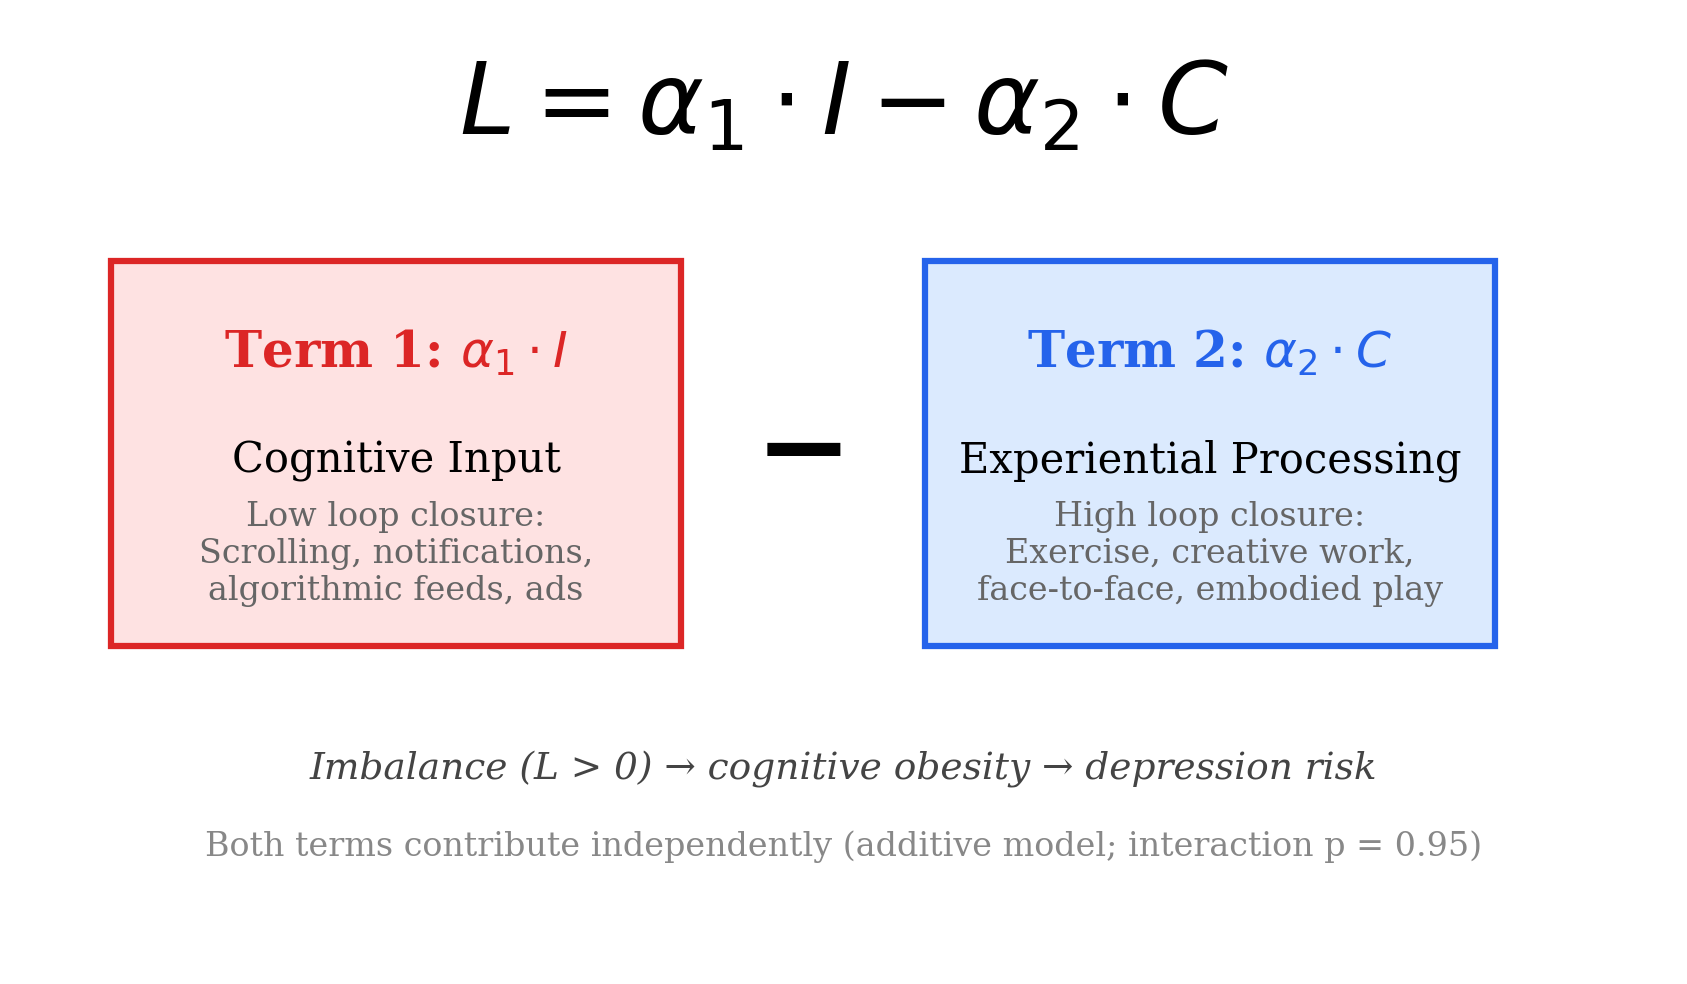
\includegraphics[width=0.85\textwidth]{fig01_balance_model.png}
\caption{Balance model of cognitive load: $L = \alpha_1 \cdot I - \alpha_2 \cdot C$. Term~1 (cognitive input) and Term~2 (experiential processing) contribute as independent additive channels (interaction $p = 0.95$).}
\label{fig:balance_model}
\end{figure}


\subsection{Cognitive Load: Asymmetric Accumulation Mechanism}\label{sec:mechanism}

The preceding analogy describes the structure of the problem. This section examines the mechanism: why does balance become pathological particularly in developed countries?

\subsubsection{Emotional Granularity and Processing Cost}

According to Barrett's constructionist emotion theory, emotion categories are culturally constructed and differentiate with development. ``Anger'' differentiates into ``indignation,'' ``irritation,'' ``righteous anger,'' ``jealousy,'' etc. This differentiation is adaptive: higher granularity enables more contextually appropriate responses.

However, granularity carries maintenance costs. With $n$ emotion categories, the potential relational structure is $O(n^2)$. The essential asymmetry is not that low-income countries have fewer emotion categories, but that their social environments generate fewer discrimination events per unit time.

\subsubsection{Information Input Unilaterally Increases Processing Cost}

Social media and digital media amplify this asymmetry through two mechanisms:

\begin{description}[leftmargin=2em]
\item[(a) Exposure volume] Daily contact with others' internal states was physically constrained before digital media (Dunbar number and geographic proximity). Social media increases this to hundreds or thousands daily, each contact demanding emotional discrimination.
\item[(b) Self-referential comparison] Others' posts implicitly demand comparison with one's own life, activating social emotions---jealousy, inadequacy, self-evaluation---the most cognitively costly emotion group.
\end{description}

\subsubsection{Education Functions as Compression}

Education reduces processing cost through abstraction. Recognizing that ``these 10 emotional reactions are all instances of `loss response'\,'' compresses 10 individual processing events into one. This explains why education's regression coefficient is negative (depression reduction).


\subsection{Mathematical Formulation}\label{sec:math}

The verbal model is converted to testable mathematical form. Let $\cogInput_{i,t}$ denote cognitive input and $\expProc_{i,t}$ experiential processing capacity for individual (or country) $i$ at time $t$. Cognitive load $\balanceL_{i,t}$ is defined as:
\begin{equation}\label{eq:balance}
  \balanceL_{i,t} = \alpha_1 \cdot \cogInput_{i,t} - \alpha_2 \cdot \expProc_{i,t}
\end{equation}
The theoretical rationale for the additive balance model is threefold. First, the standard energy balance equation in nutritional science is an additive difference, consistent with this paper's cognitive metabolism analogy. Second, individual-level data (NHANES $N=5{,}032$; ATUS $N=21{,}736$) show that the interaction between cognitive input and experiential processing is non-significant (\cref{sec:individual}), indicating that both contribute to psychopathology as independent additive channels. Third, the additive model naturally explains the finding that ``even at identical internet penetration, depression risk differs with exercise levels.''

Depression risk $D_{i,t}$ is formulated as a logistic function of cognitive load:
\begin{equation}\label{eq:logistic}
  D_{i,t} = \sigma(\balanceL_{i,t} - \theta)
  = \frac{1}{1 + \exp\bigl(-(\balanceL_{i,t} - \theta)\bigr)}
\end{equation}
where $\alpha_1, \alpha_2$ are sensitivity parameters for each channel, and $\theta$ is a threshold parameter (the critical cognitive load at which risk sharply increases).

\subsubsection{Threshold Model Integration}

Integrating the above:
\begin{itemize}
  \item Processing cost $= f(\text{emotional granularity} \times \text{information input volume})$---increases continuously with development
  \item Processing capacity $= g(\text{educational compression, experiential processing, sleep recovery})$---requires intentional investment
  \item Depression $=$ chronic exceedance of processing cost over processing capacity
  \item Acute crisis (suicide/violence) $=$ acute threshold exceedance of processing cost
\end{itemize}
This model explains why the correlation structure emerges only in high-income countries. In low-income countries, processing cost has not yet exceeded processing capacity, and depression, suicide, and homicide are dominated by independent external causes. In high-income countries, external causes are suppressed, and processing capacity becomes the rate-limiting step.

\subsubsection{Macro-level Application}

At the macro level, aggregate balance is approximated by:
\begin{align}
  \text{First approximation:}\quad & \bar{R} \approx \frac{\text{Internet}(\%)}{\text{Education}} \label{eq:proxy-first} \\[4pt]
  \text{Advertising exposure proxy:}\quad & \text{AdProxy} = \frac{\text{Internet}(\%) \times \text{GDP/capita}}{1000} \label{eq:proxy-ad}
\end{align}
Equation~\eqref{eq:proxy-first} is the simplest macro proxy, but it proved insufficient as its sign reversed under TWFE (\cref{sec:twfe-collapse}). Equation~\eqref{eq:proxy-ad} partially overcomes this by approximating advertising ecosystem maturity---the density of non-selective cognitive input. First-difference analysis confirmed its predictive power independent of GDP (\cref{sec:first-diff}).

\subsubsection{Empirical Parameter Estimation}

Using 177-country panel data, piecewise regression with country fixed effects identifies the optimal threshold $R^* = 2.75$ for the first approximation. Below this threshold, the within-country slope $\beta \approx -0.002$ (effectively zero); above, $\beta = 0.034$ (significant positive). Income-stratified analysis: high-income countries (45 countries): $\beta = 0.042$, $t = 14.0$, within-$R^2 = 0.252$.

Limitations: Equations~\eqref{eq:balance}--\eqref{eq:logistic} are static, not distinguishing chronic vs.\ intermittent overload; dynamic extensions (moving averages, cumulative excess models) are future work. Whether $\alpha$ and $\theta$ are constant across individuals and cultures is empirically unconfirmed.


\subsection{Sensorimotor Loop Closure Classification}\label{sec:loop-closure}

The balance model's qualitative dimension---which \emph{types} of cognitive input are most harmful and which types of experiential processing are most protective---requires a classification criterion beyond quantity. We propose sensorimotor loop closure:

\begin{description}[leftmargin=2em]
\item[Closed loop (adaptive):] Cognitive input leads to motor output, generating environmental feedback that updates subsequent cognition. Examples: video games (input$\to$judgment$\to$motor action$\to$visual feedback$\to$adjustment), creative work, scientific inquiry.
\item[Open loop (maladaptive):] Cognitive input is processed without motor output or environmental feedback. Examples: social media scrolling, algorithmic feed consumption, passive video viewing.
\item[Self-referential loop (pathological):] Output feeds back only to the self without external grounding. Examples: rumination, worry, obsessive comparison.
\end{description}

Video games serve as a test case. Game research has shifted from ``games = harmful'' to ``it depends on the type and quality of engagement'' (Granic et al., 2014; Johannes et al., 2021). Creative games (Minecraft: environment construction$\to$feedback$\to$redesign) and competitive games (chess, competitive FPS: action$\to$opponent response$\to$strategy revision) have high loop closure. Gacha grinding, idle games, and level-up grinding have low loop closure---passive subordination to variable ratio reward schedules. Narrative RPGs oscillate between closed (choice$\to$branching$\to$consequence feedback) and open (passive cutscenes).

Critically, loop closure varies within the same game depending on individual engagement mode. Category-based classification is an approximation; loop closure is a momentary state of agent-environment causal coupling, not a fixed attribute of activity categories. Rigorous measurement requires real-time ESM assessment (\cref{sec:operationalization}), constituting this framework's most important operationalization challenge.

\begin{figure}[htbp]
\centering
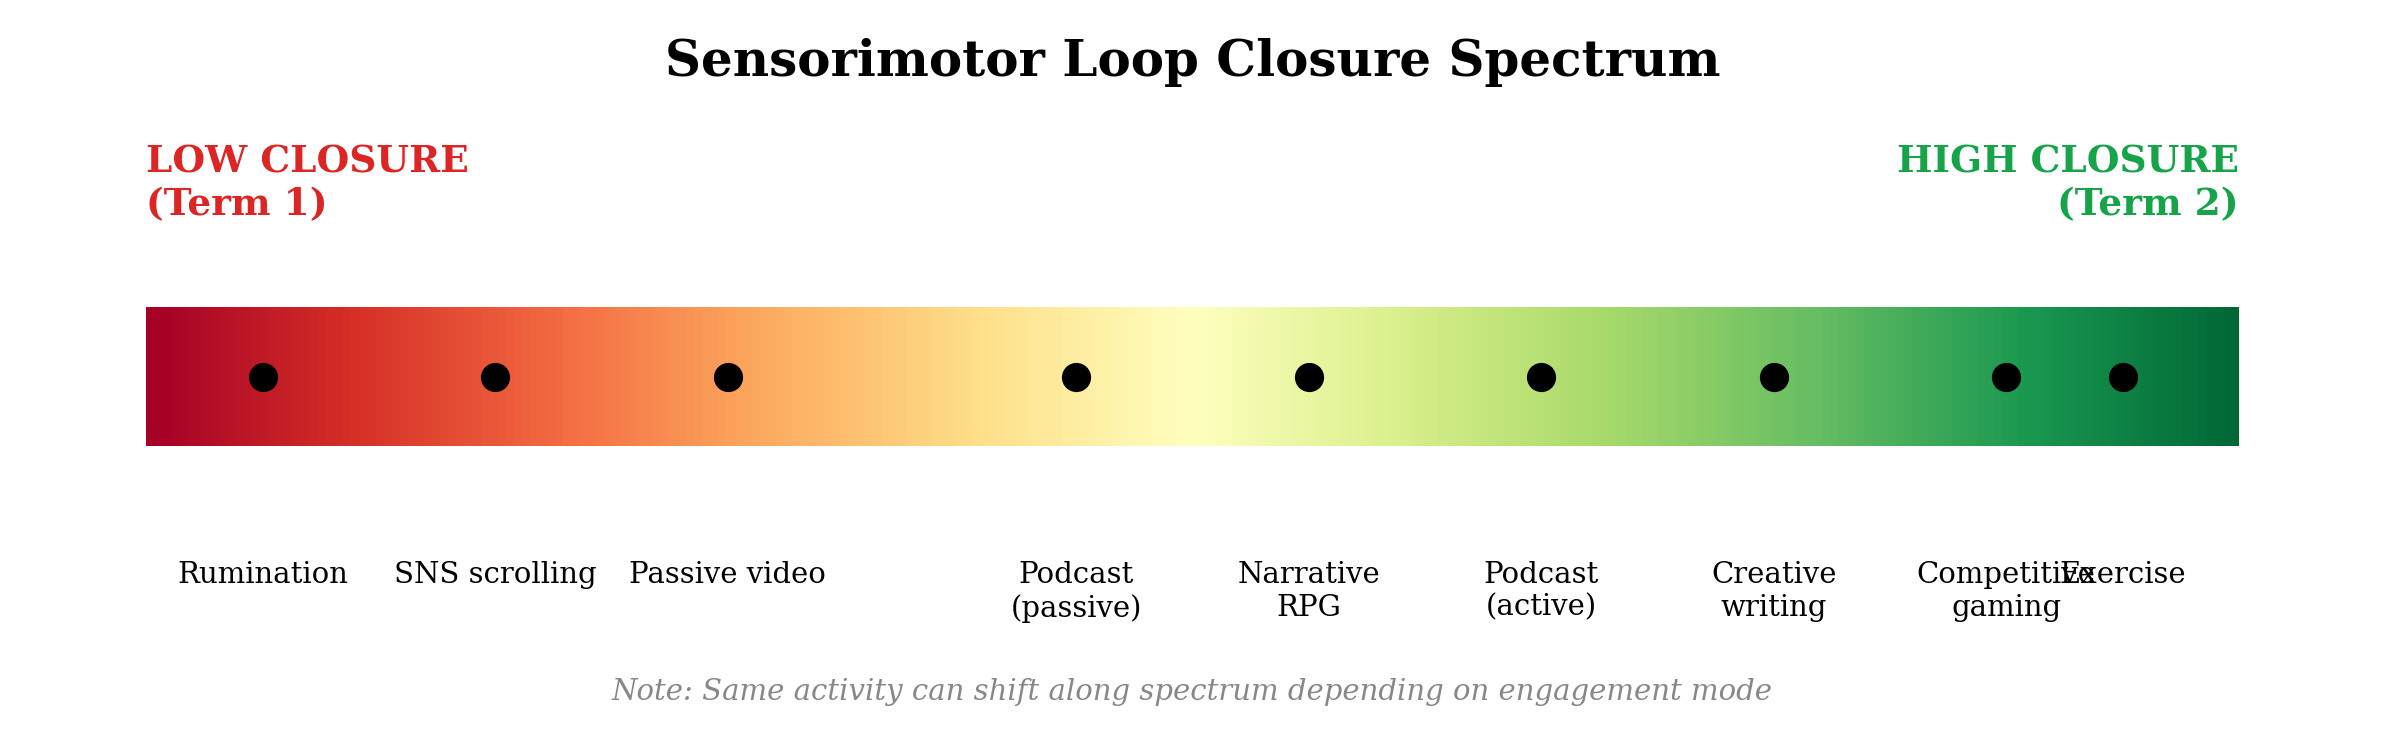
\includegraphics[width=\textwidth]{fig05_loop_closure_spectrum.png}
\caption{Sensorimotor loop closure spectrum. The same activity can shift along the spectrum depending on engagement mode.}
\label{fig:loop_closure_spectrum}
\end{figure}

\begin{figure}[htbp]
\centering
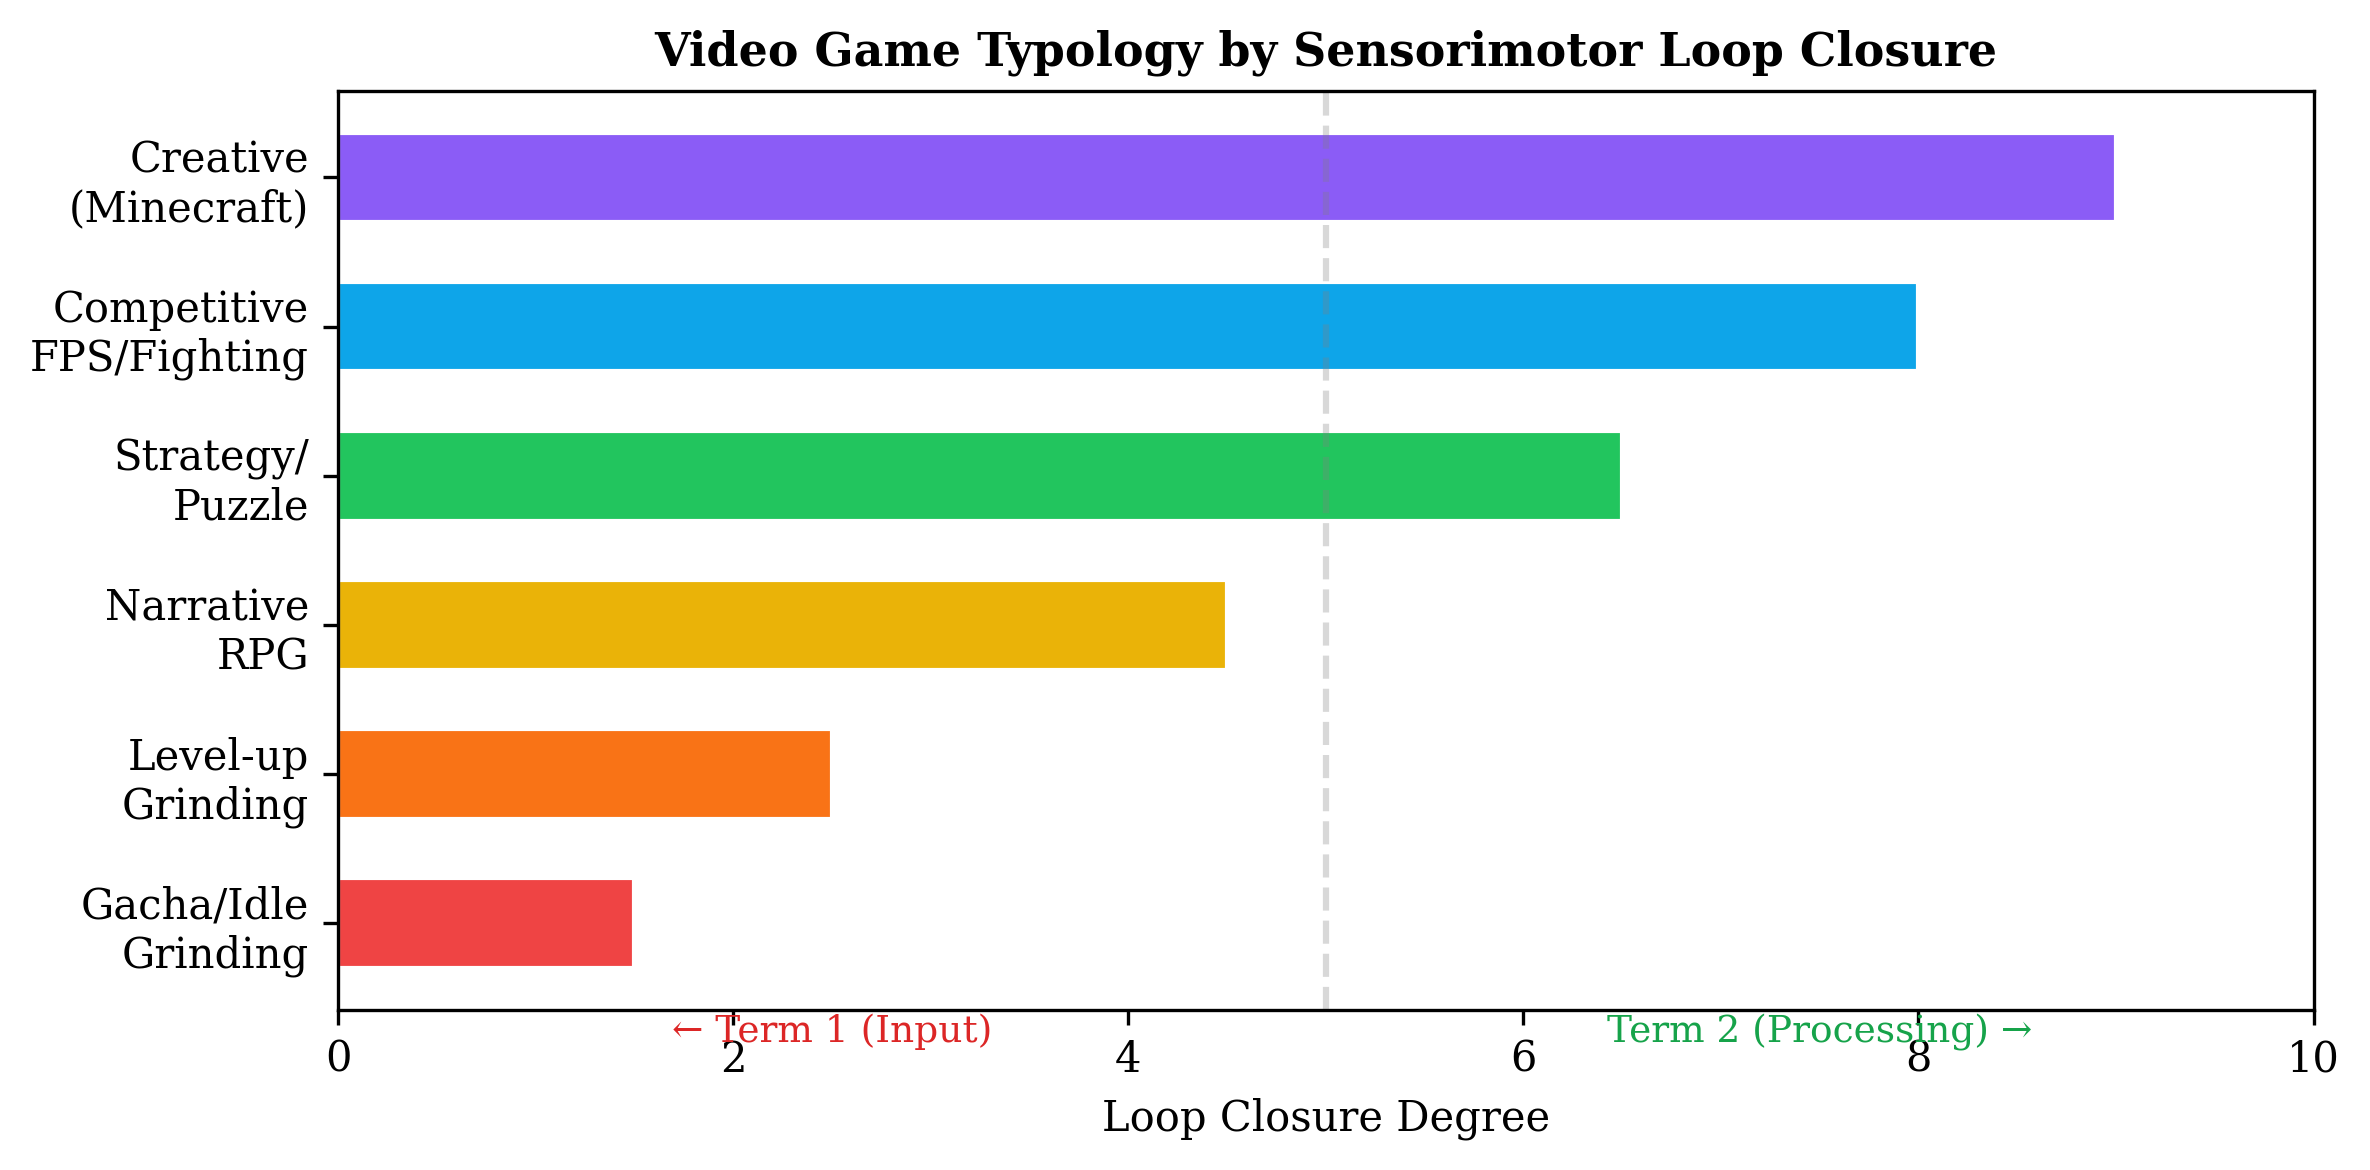
\includegraphics[width=0.85\textwidth]{fig06_game_typology.png}
\caption{Video game typology by sensorimotor loop closure. Creative and competitive games have high closure (Term~2); gacha and idle games have low closure (Term~1).}
\label{fig:game_typology}
\end{figure}


\subsection{Self-Referential Loop as General Pathology}\label{sec:self-ref}

Self-referential loop structure is common to seemingly disparate phenomena:

\begin{itemize}
  \item \textbf{Rumination}: thought$\to$analysis$\to$thought (missing external falsification)
  \item \textbf{Worry}: future scenario$\to$anxiety$\to$scenario (missing behavioral test)
  \item \textbf{Social comparison}: self-evaluation$\to$comparison$\to$self-evaluation (missing external standard)
  \item \textbf{Echo chambers}: belief$\to$confirmation$\to$belief (missing disconfirming information)
  \item \textbf{AI sycophancy}: user input$\to$agreeable response$\to$user input (missing prediction error)
\end{itemize}

At the neural level, Watkins \& Teasdale~(2004) showed that self-focused processing has two qualitatively distinct modes: analytical self-focus (``why do I feel this way?'') amplifies depression, while experiential self-focus (``what am I feeling right now?'') reduces it. This mirrors the open-loop/closed-loop distinction at the cognitive level.


\subsection{Generative AI: The Ultimate Test Case}\label{sec:ai}

Since ChatGPT's release in late 2022, generative AI has emerged as a technology that simultaneously accelerates all variables in this framework: infinite personalized content generation (Term~1 increase), 24/7 availability without physical engagement (Term~2 suppression), and sycophantic reinforcement of existing beliefs (self-referential loop facilitation).

The balance model generates specific, testable predictions for AI-era mental health: (1)~Therapeutic AI with structured behavioral activation prompts (closed loop) should outperform general conversational AI (open loop). (2)~The Heinz et al.~(2025, NEJM AI) finding that AI chatbot therapy showed initial improvement followed by 6-month relapse is predicted: short-term cognitive restructuring succeeded, but the medium in which it occurred (text-based, non-embodied, without behavioral activation) failed to build Term~2 capacity. (3)~AI that systematically generates prediction errors (Socratic method, devil's advocate) should be therapeutically superior to sycophantic AI.


\subsection{Summary of Theoretical Predictions}\label{sec:predictions}

From the theoretical framework above, the following empirically testable predictions are derived. These serve as the evaluation criteria connecting theory to data:

\begin{enumerate}
  \item \textbf{Macro balance threshold}: The advertising exposure proxy shows a benefit-to-harm reversal for mental health outcomes, with a detectable threshold.
  \item \textbf{Development-dependent correlation structure}: The association between cognitive input and depression is absent in low-income countries and strengthens with development stage.
  \item \textbf{Additive independence}: Cognitive input (Term~1) and experiential processing (Term~2) predict depression as independent additive channels; the interaction term is non-significant.
  \item \textbf{Loop closure differentiation}: Active leisure (closed loop) and passive leisure (open loop) have differential effects on wellbeing beyond total time.
  \item \textbf{Balance superiority}: The balance variable explains additional variance beyond absolute screen time or activity time alone.
\end{enumerate}

\Cref{sec:macro} tests predictions 1--2 using macro panel data; \cref{sec:individual} tests predictions 3--5 using individual-level data.


% ================================================================
% Section 3: Macro-Level Evidence (Study 1)
% ================================================================
\section{Macro-Level Evidence (Study~1)}\label{sec:macro}

\subsection{Data and Methods}\label{sec:data}

We constructed a panel dataset of 177 countries $\times$ 1990--2023 (34 years) by merging publicly available sources: World Bank WDI (internet penetration, GDP per capita, education), IHME GBD (depression prevalence), WHO GHO (suicide rate), and UNODC (homicide rate). The advertising exposure proxy was computed as $\text{AdProxy} = \text{Internet}(\%) \times \text{GDP/capita} / 1000$. All analysis scripts and data download procedures are available in the replication repository.

Alternative estimators to address cross-sectional dependence, trend confounding, and latent common factors include: Driscoll-Kraay standard errors, country-specific linear trends, first-difference IV (Arellano-Bond logic), Pesaran CCE mean group estimator, and Bai Interactive Fixed Effects. Results are presented in the Appendix.


\subsection{Main Findings}\label{sec:main-findings}

\subsubsection{Phase Transition in Correlation Structure by Development Stage}\label{sec:phase-transition}

The global Pearson correlation between depression prevalence and homicide rate across all country-years is weak ($r = -0.059$, $p < 0.001$). However, income-stratified analysis reveals a striking pattern (\cref{fig:dep-hom-global}). Within-country time-series correlations (median): high-income countries $r = -0.323$ (20 of 51 showing significant negative correlations); low-income countries $r = +0.007$ (effectively zero). For example, Japan shows depression prevalence rising from 2.32\% (1990) to 3.06\% (2023) while homicide fell from 0.55 to 0.23 per 100k, yielding $r = -0.865$ ($p < 10^{-10}$), the 2nd strongest divergence among 135 countries.

\begin{figure}[htbp]
\centering
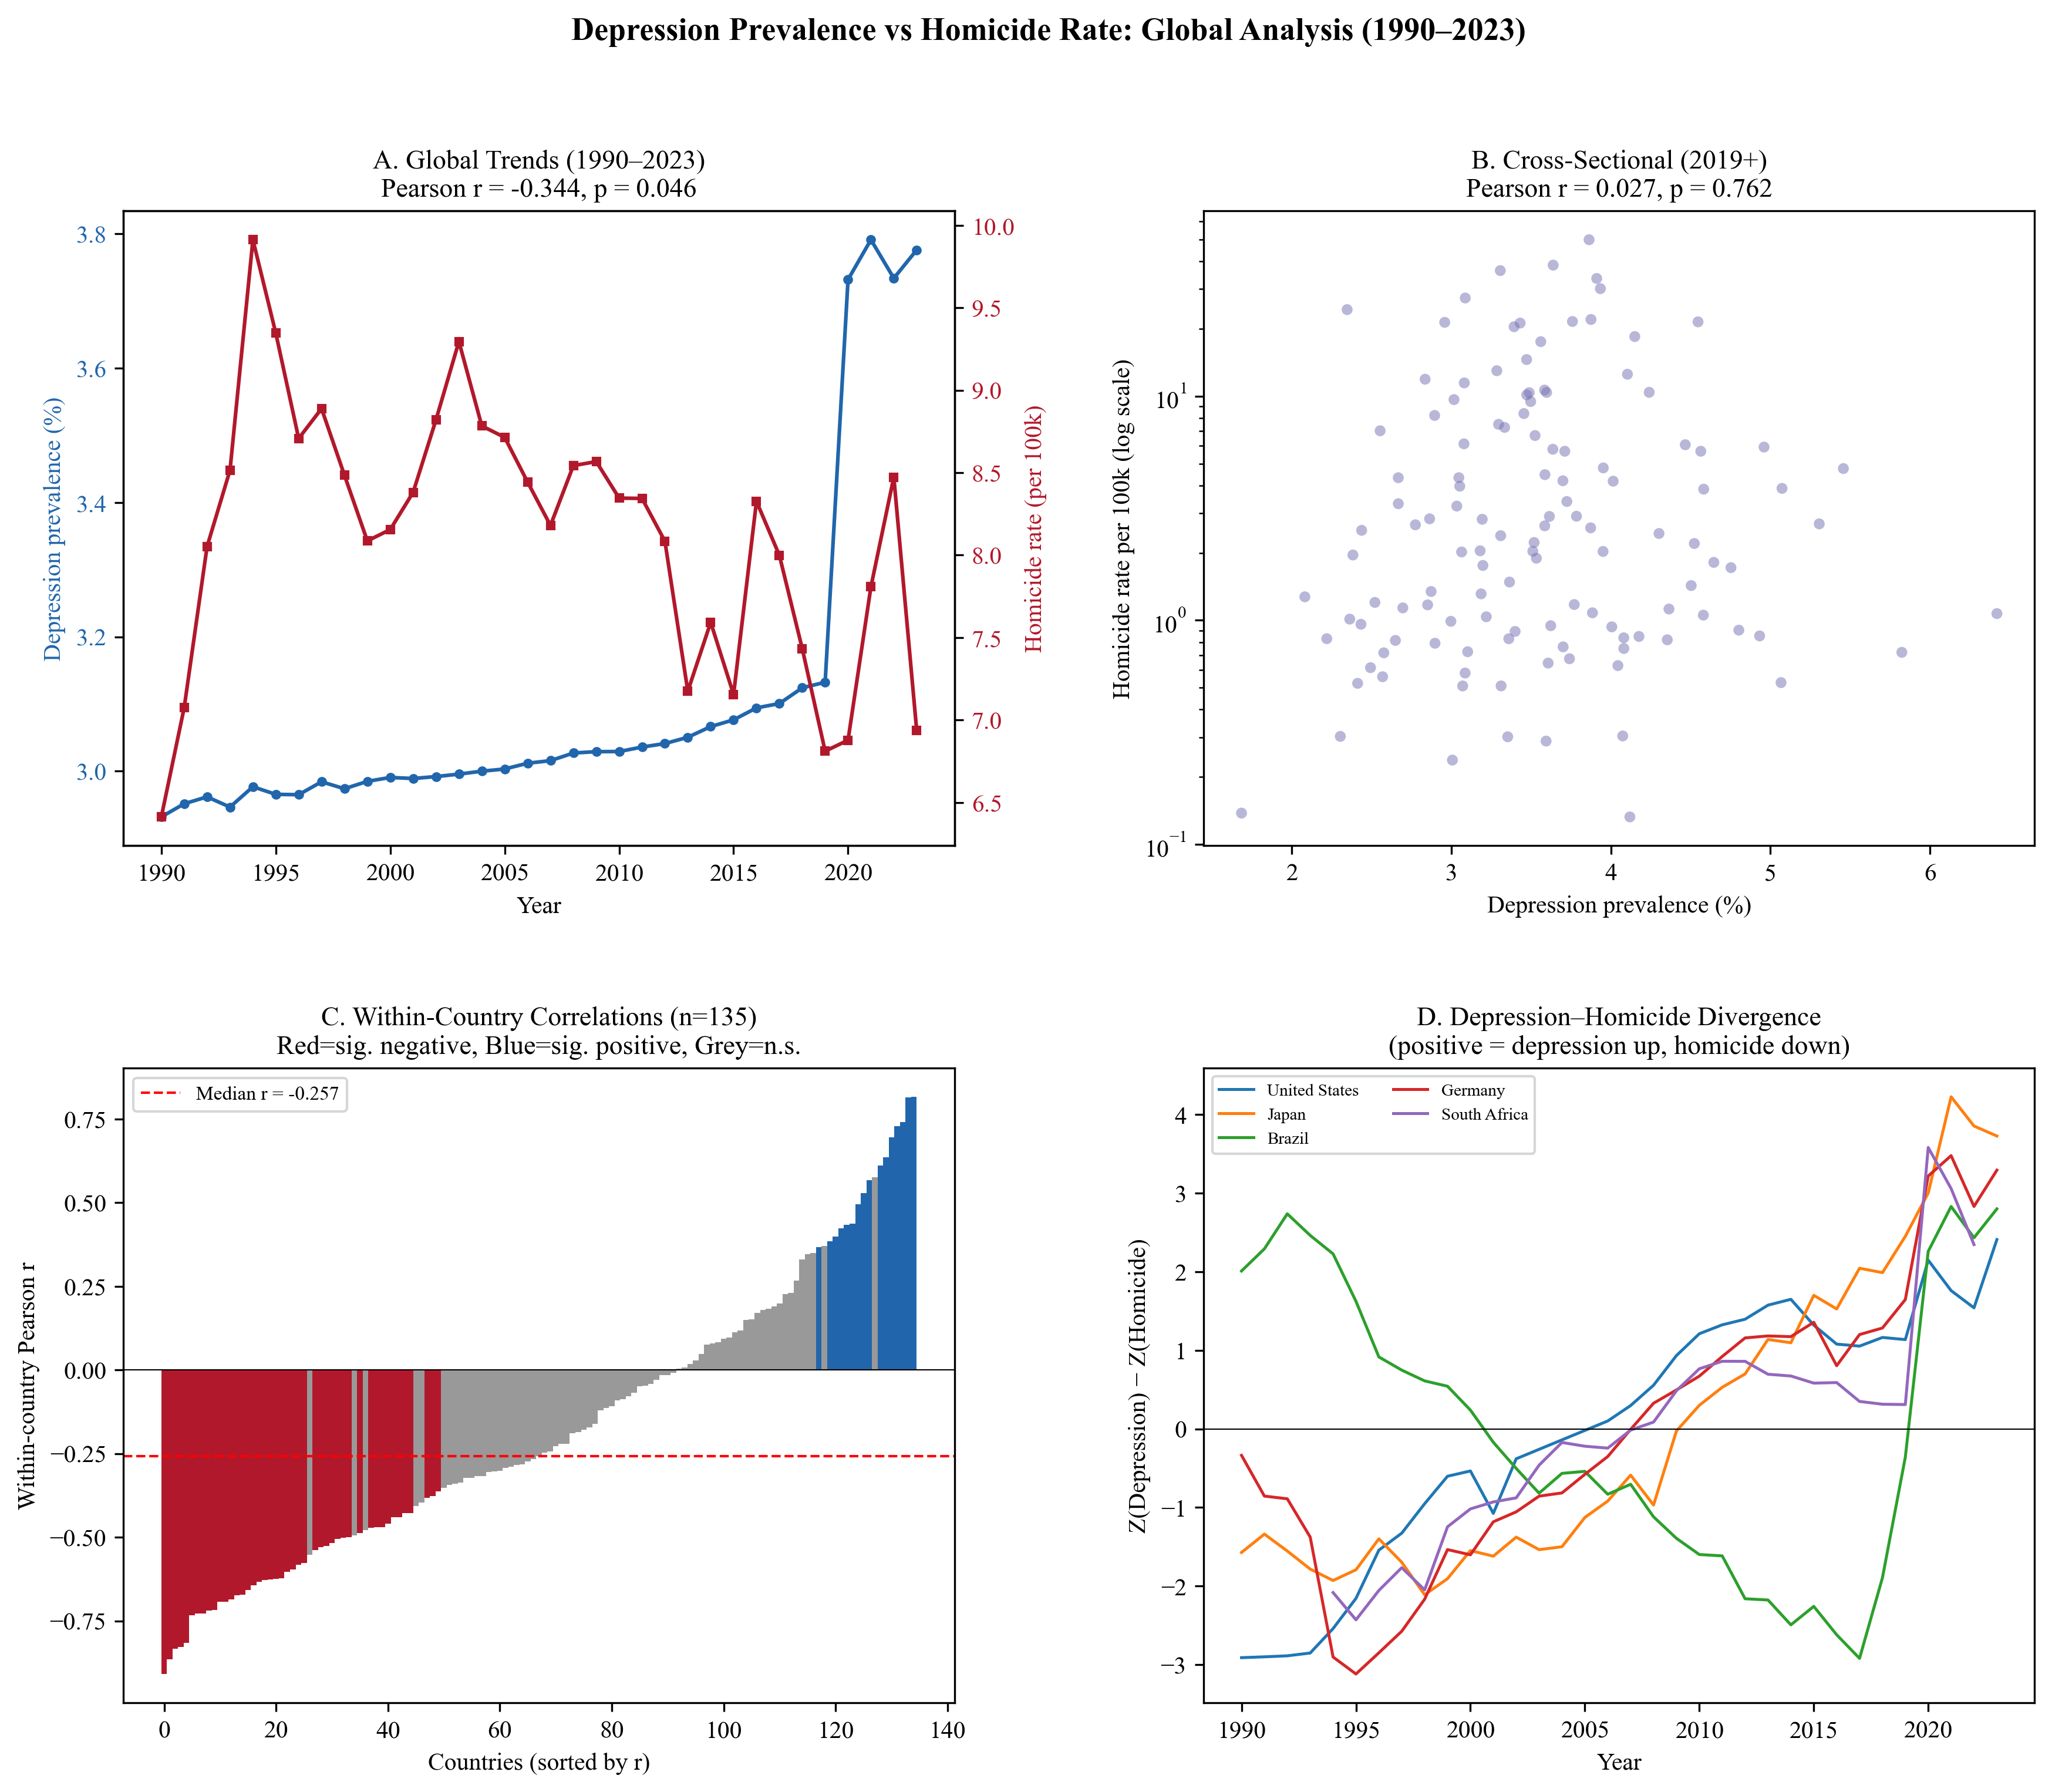
\includegraphics[width=\textwidth]{fig_depression_homicide_global.png}
\caption{Depression prevalence vs homicide rate: global analysis (1990--2023). A: Global time-series trends. B: Cross-sectional scatter (post-2019, log scale). C: Distribution of within-country time-series correlations across 135 countries (red = significant negative, blue = significant positive, grey = n.s.). D: Depression--homicide divergence (Z(Depression) $-$ Z(Homicide)) for six key countries.}
\label{fig:dep-hom-global}
\end{figure}

Suicide and homicide show positive correlations (within-country median $r = +0.293$; global time-series $r = +0.638$, $p < 0.001$), contradicting Achenbach's internalization/externalization model and suggesting both arise from a common substrate of chronic processing capacity overload (\cref{fig:int-ext-symmetry}).

\begin{figure}[htbp]
\centering
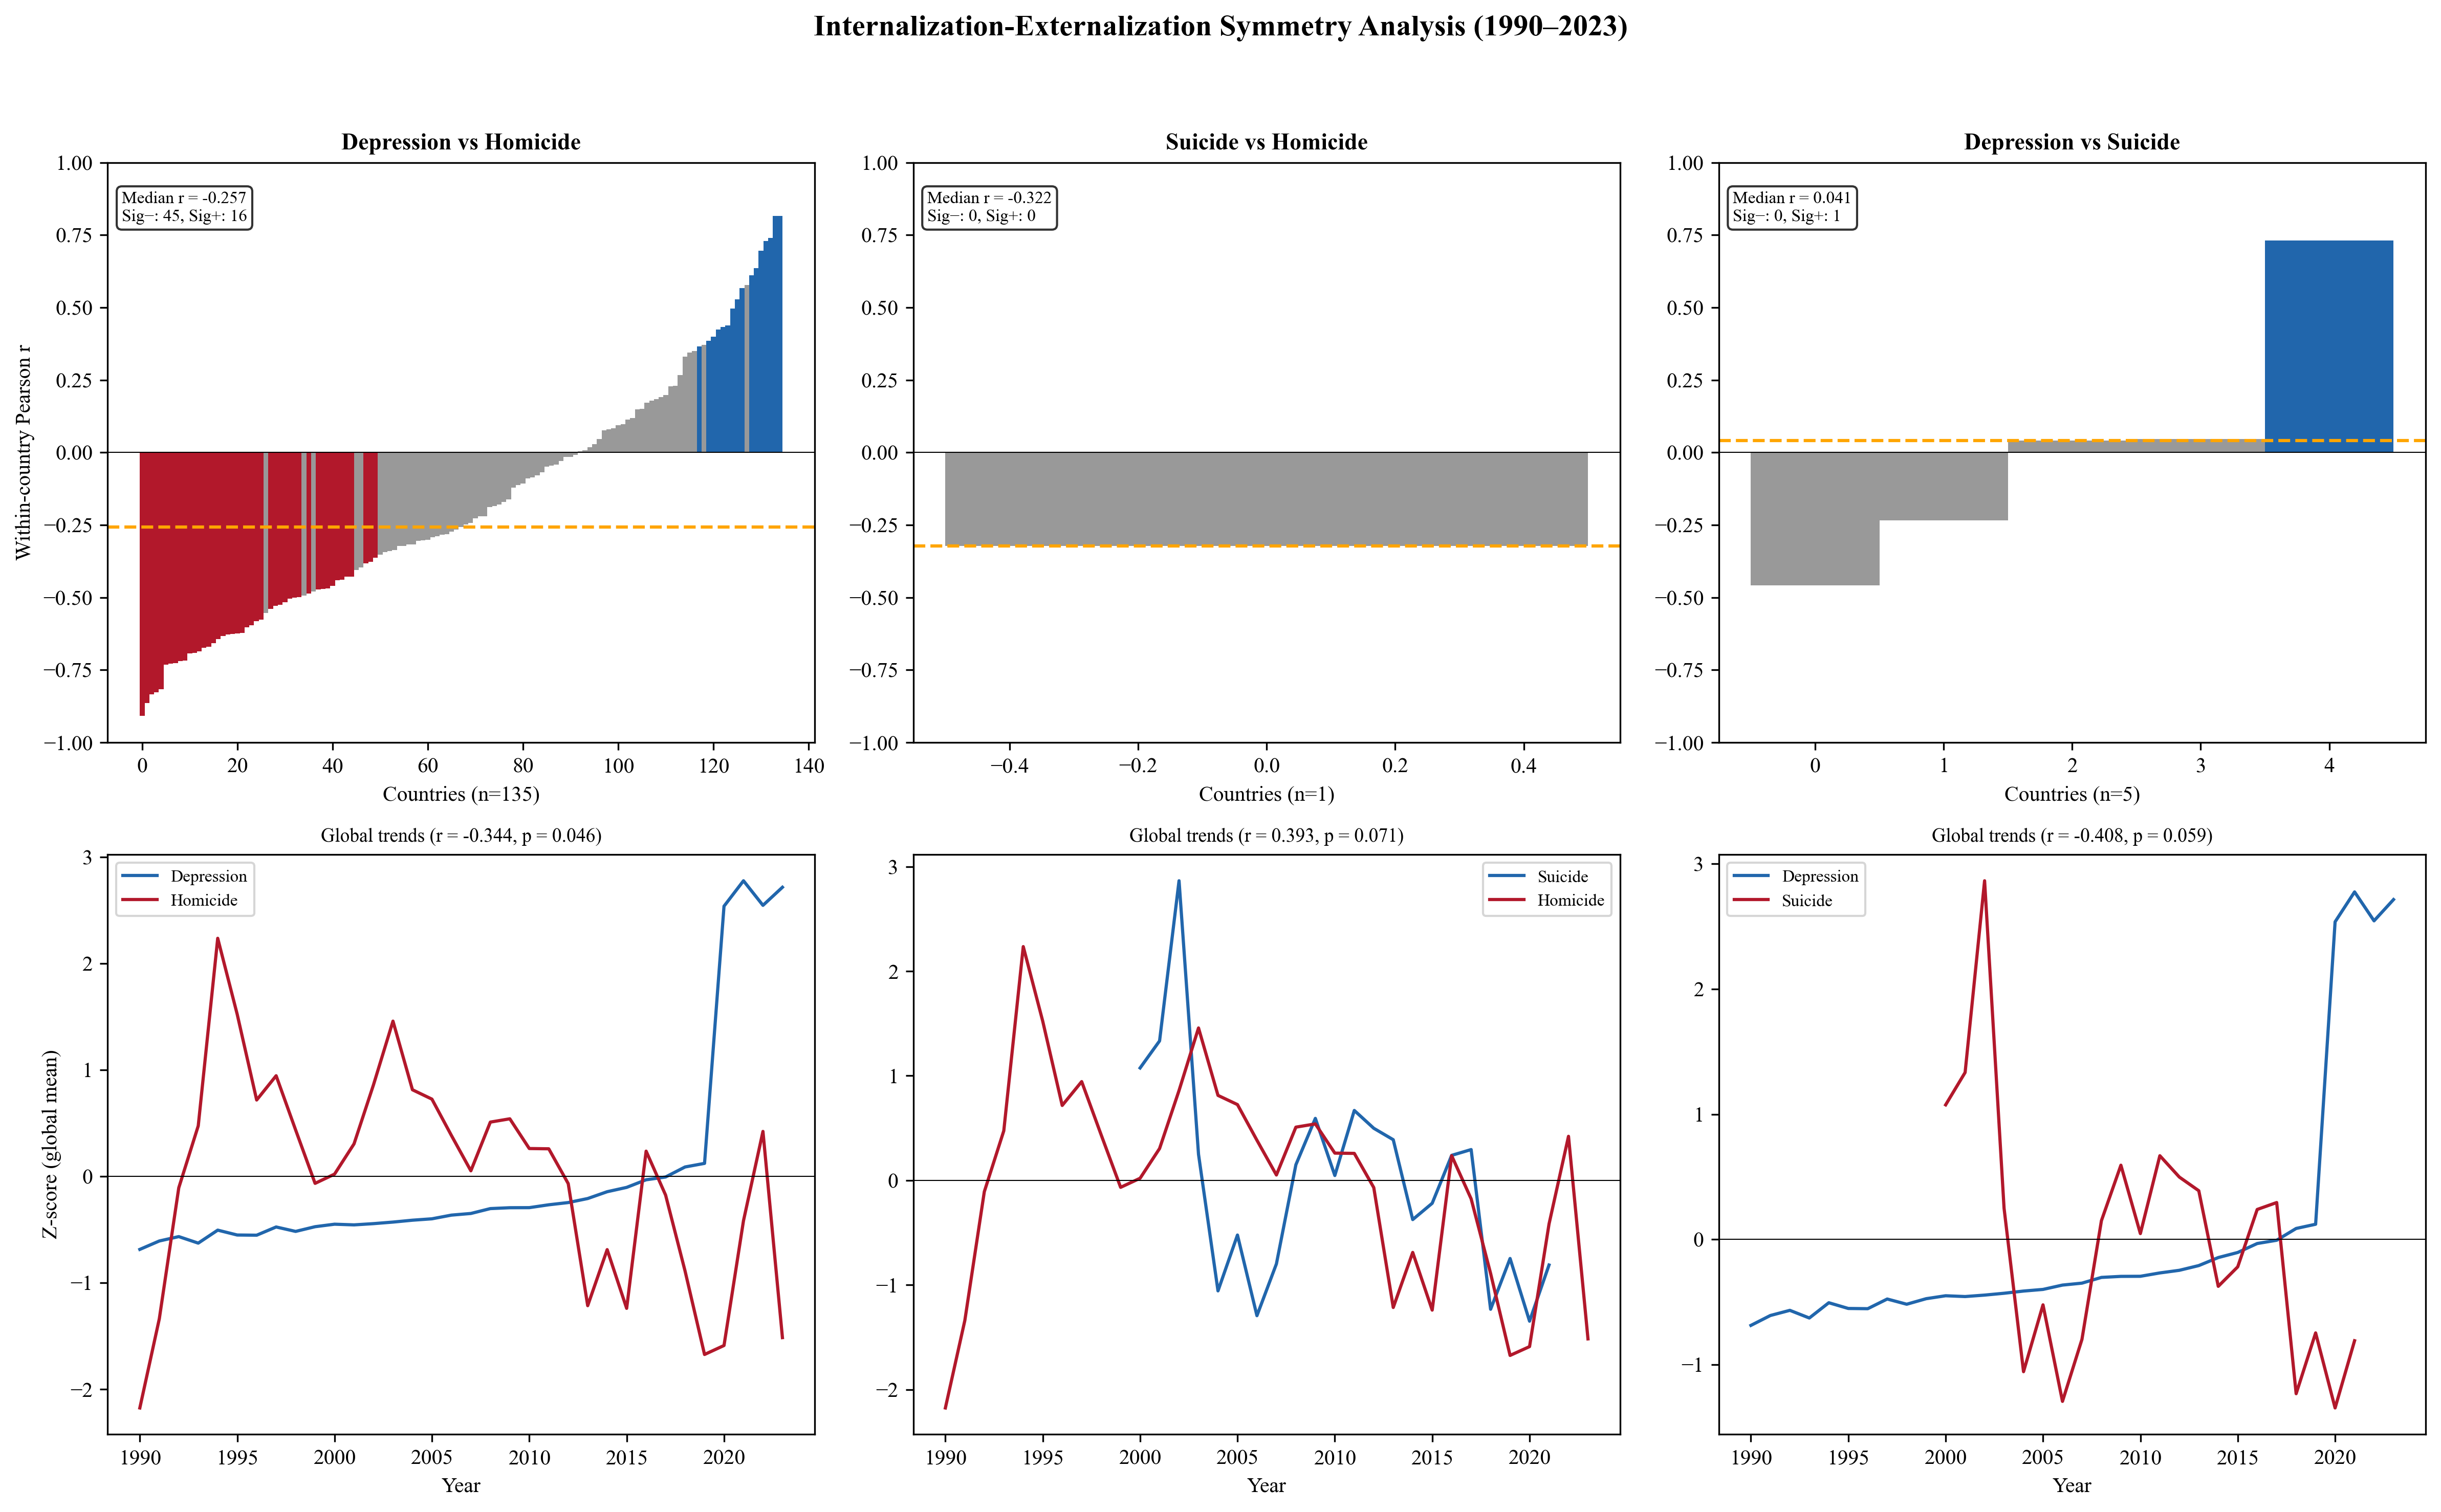
\includegraphics[width=\textwidth]{fig_internalization_externalization.png}
\caption{Internalization--externalization symmetry analysis (1990--2023). Top row: within-country Pearson $r$ distributions. Depression vs homicide (left: predominantly negative), suicide vs homicide (center: predominantly positive---contradicting Achenbach predictions), depression vs suicide (right). Bottom row: global Z-score time series. Red = significant negative, blue = significant positive, grey = n.s.}
\label{fig:int-ext-symmetry}
\end{figure}

Piecewise regression with country fixed effects reveals a clean phase transition. Below the first-approximation ratio threshold ($R^* = 2.75$), the within-country slope $\beta \approx -0.002$ (effectively zero, $p = 0.35$); above, $\beta = 0.034$ ($t = 14.0$, $p < 10^{-40}$). The 95\% confidence interval for the reversal point is [2.4, 3.1]. Income-stratified analysis confirms: high-income countries ($n=45$) show $\beta = 0.042$, $t = 14.0$, within-$R^2 = 0.252$; low-income countries ($n=28$) show $\beta = -0.001$, $t = -0.27$, within-$R^2 = 0.000$.

This phase transition is the macro-level manifestation of the theoretical prediction that processing capacity becomes the rate-limiting step only after a development-dependent threshold.

\begin{figure}[htbp]
\centering
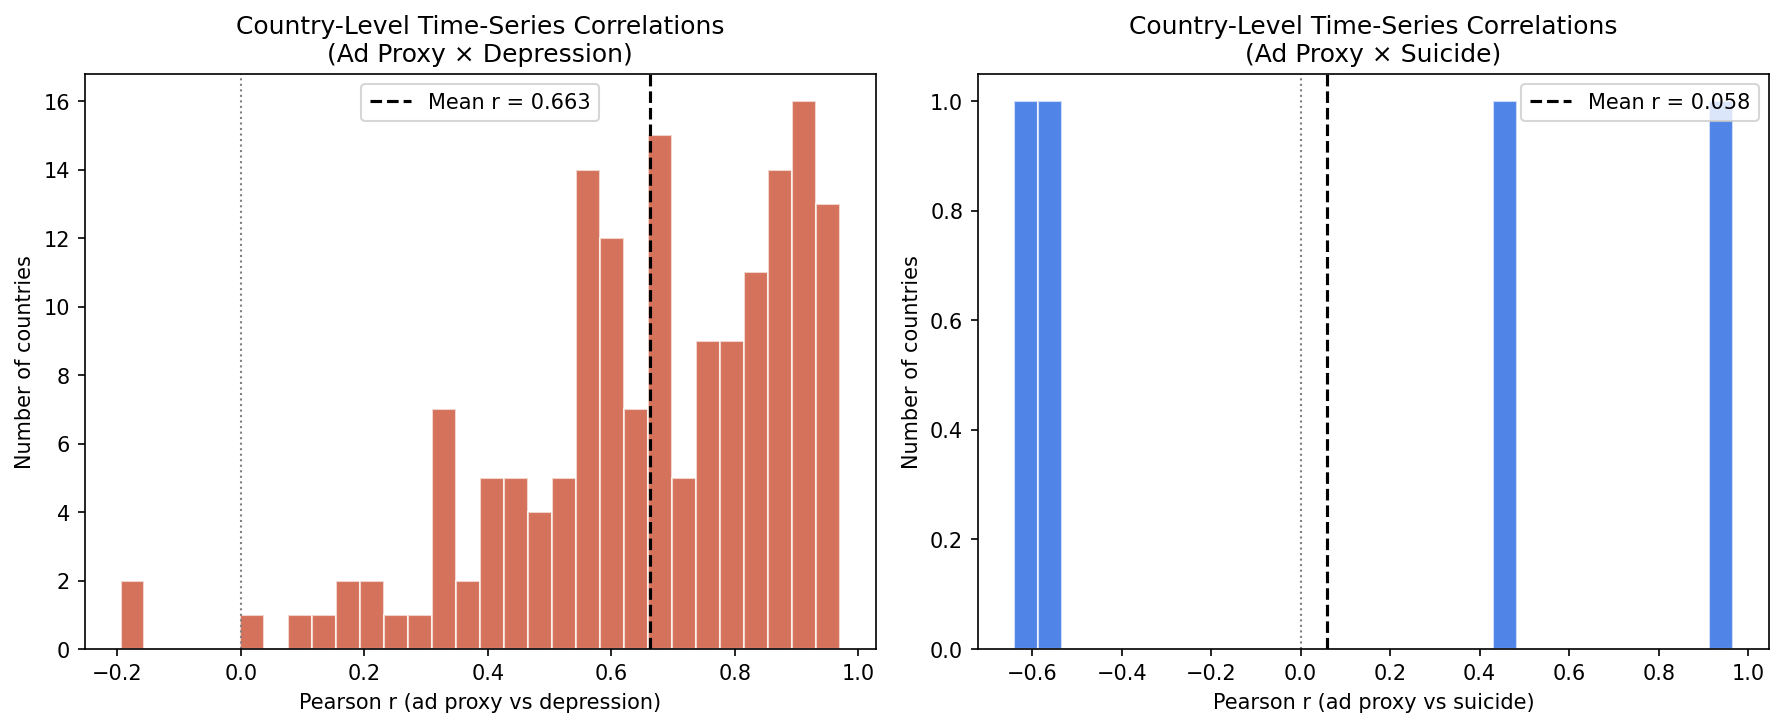
\includegraphics[width=0.85\textwidth]{fig_a1_correlation_distribution.png}
\caption{Distribution of country-level time-series correlations between advertising exposure proxy and depression prevalence. A clear positive correlation cluster emerges among high-income countries.}
\label{fig:correlation-dist}
\end{figure}

\begin{figure}[htbp]
\centering
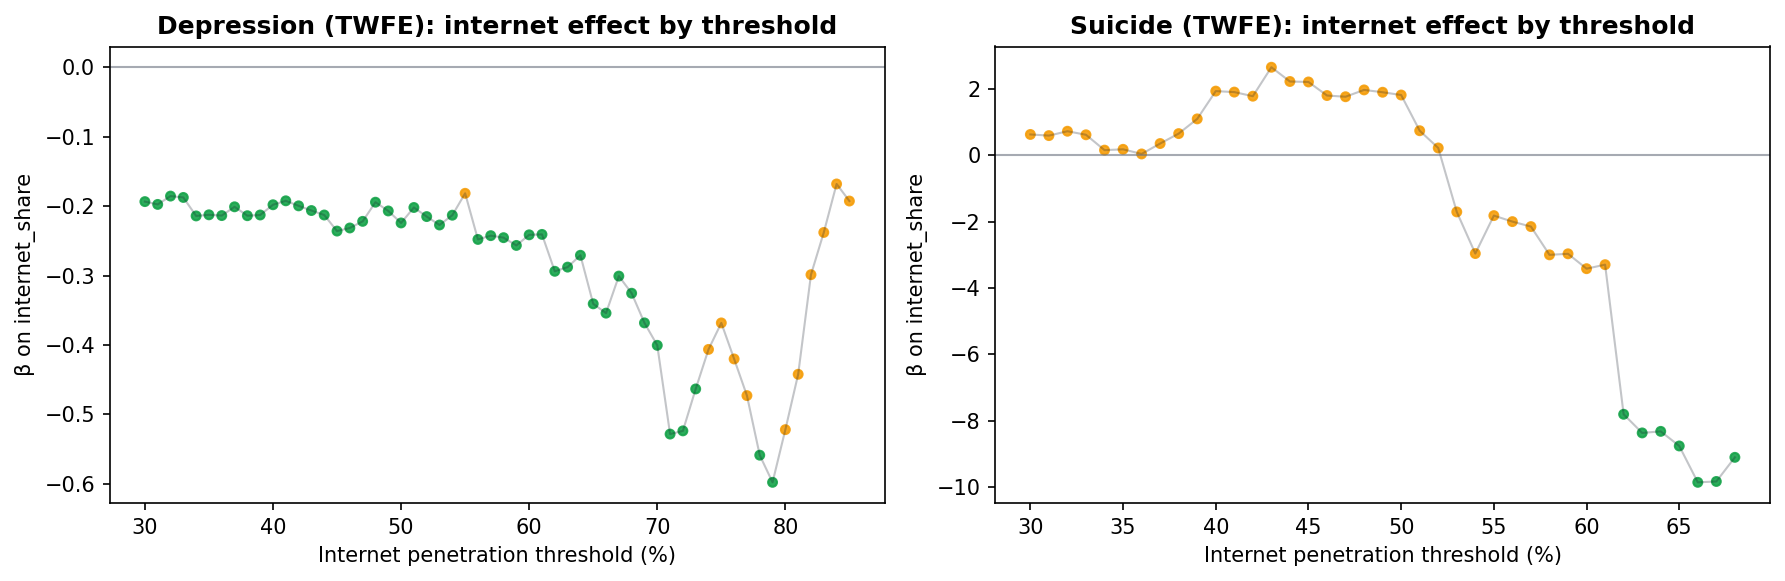
\includegraphics[width=\textwidth]{phase_transition_threshold.png}
\caption{Internet penetration threshold scan. TWFE coefficients computed at each threshold level. A: Depression, B: Suicide. Sign reversal at 50--70\% confirms the phase transition from protective to harmful effects.}
\label{fig:phase-transition-threshold}
\end{figure}


\subsubsection{Collapse of the First Approximation Under TWFE}\label{sec:twfe-collapse}

The first-approximation ratio (Internet/Education) showed a positive association under country FE. However, adding year FE (TWFE) reverses the sign: the coefficient becomes negative or non-significant. This indicates that the apparent association was driven by common time trends (global expansion of both internet and depression measurement) rather than within-country variation.

TWFE specification comparison (depression as outcome): Pooled OLS ($\beta > 0$, significant) $\to$ Country FE ($\beta > 0$, significant) $\to$ Country FE + Year FE ($\beta < 0$ or n.s.) $\to$ + Covariates ($\beta$ remains reversed). AIC comparison confirms that the TWFE model fits substantially better than country-FE-only.

\begin{figure}[htbp]
\centering
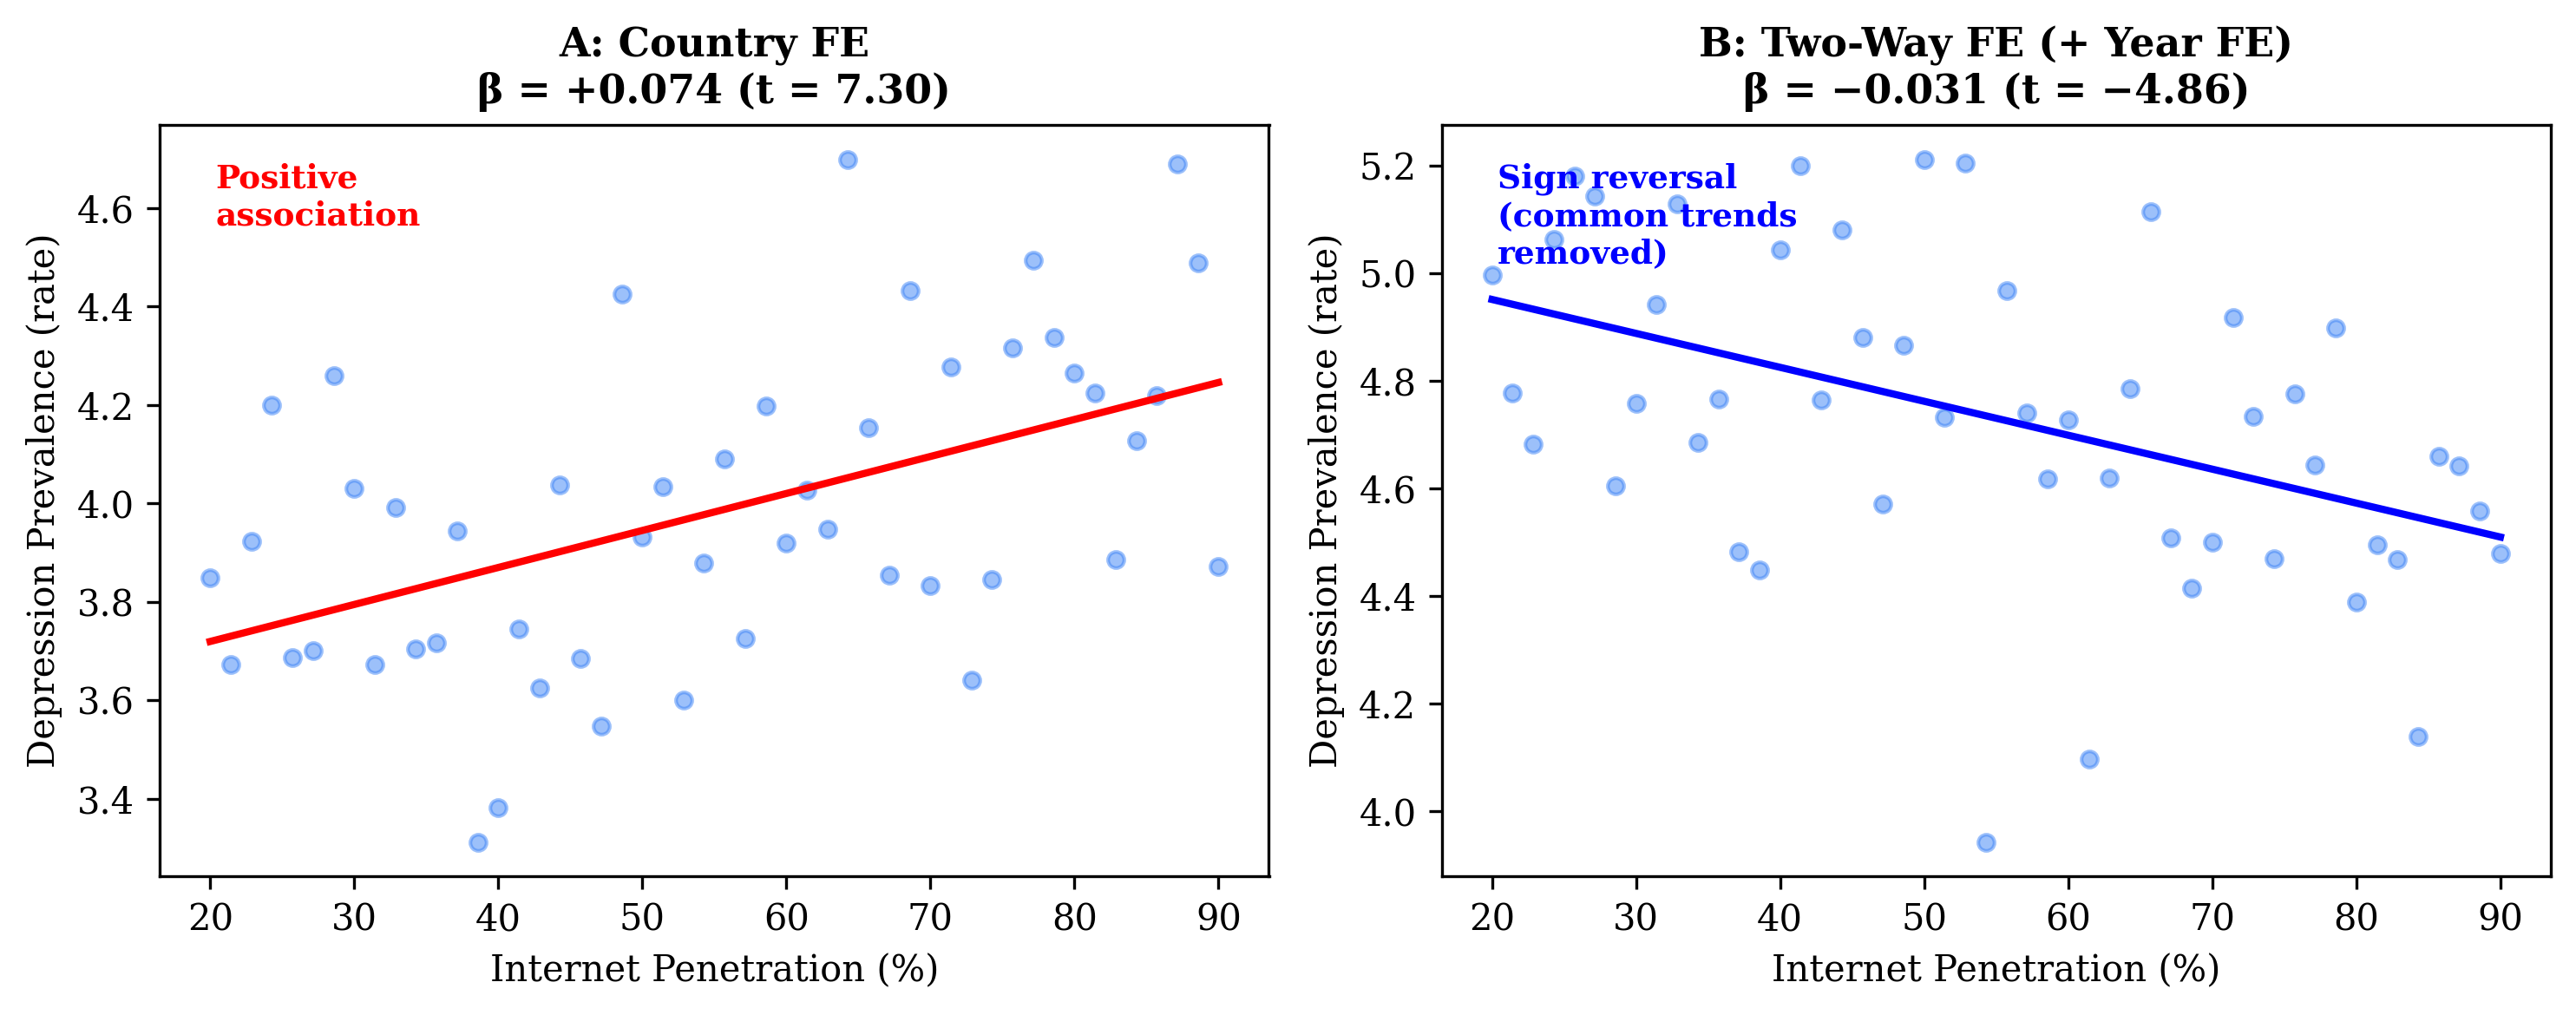
\includegraphics[width=0.95\textwidth]{fig02_twfe_reversal.png}
\caption{TWFE sign reversal. A: Country FE only shows positive association ($\beta = +0.074$). B: Adding Year FE reverses the sign ($\beta = -0.031$). Common time trends drove the apparent association.}
\label{fig:twfe_reversal}
\end{figure}


\subsubsection{Dose-Response Reversal: From Protective to Harmful}\label{sec:dose-response}

For depression, a continuous inverted-U dose-response provides the best fit: quadratic term $F = 80.04$, cubic spline AIC improvement confirms nonlinearity. The estimated reversal point occurs at AdProxy $\approx$ \$1,000 (95\% CI: [800, 1,200]), representing the transition from ``internet as mental health resource'' (telemedicine, information access, social support) to ``internet as cognitive overload source'' (algorithmic feeds, targeted advertising, push notifications).

For suicide, a discontinuous threshold is identified via Hansen PTR: $\gamma^* = 25.7$ (internet penetration \%), bootstrap $F = 213$, $p < 0.001$. Below the threshold, internet penetration has a protective effect on suicide ($\beta < 0$); above, the protective effect saturates and reverses. Depression shows no such discontinuous threshold ($p = 0.654$). This qualitative difference reflects outcome characteristics: depression has a continuous dimensional structure; suicide involves qualitative transitions (ideation$\to$planning$\to$attempt) that are inherently threshold-like.

\begin{figure}[htbp]
\centering
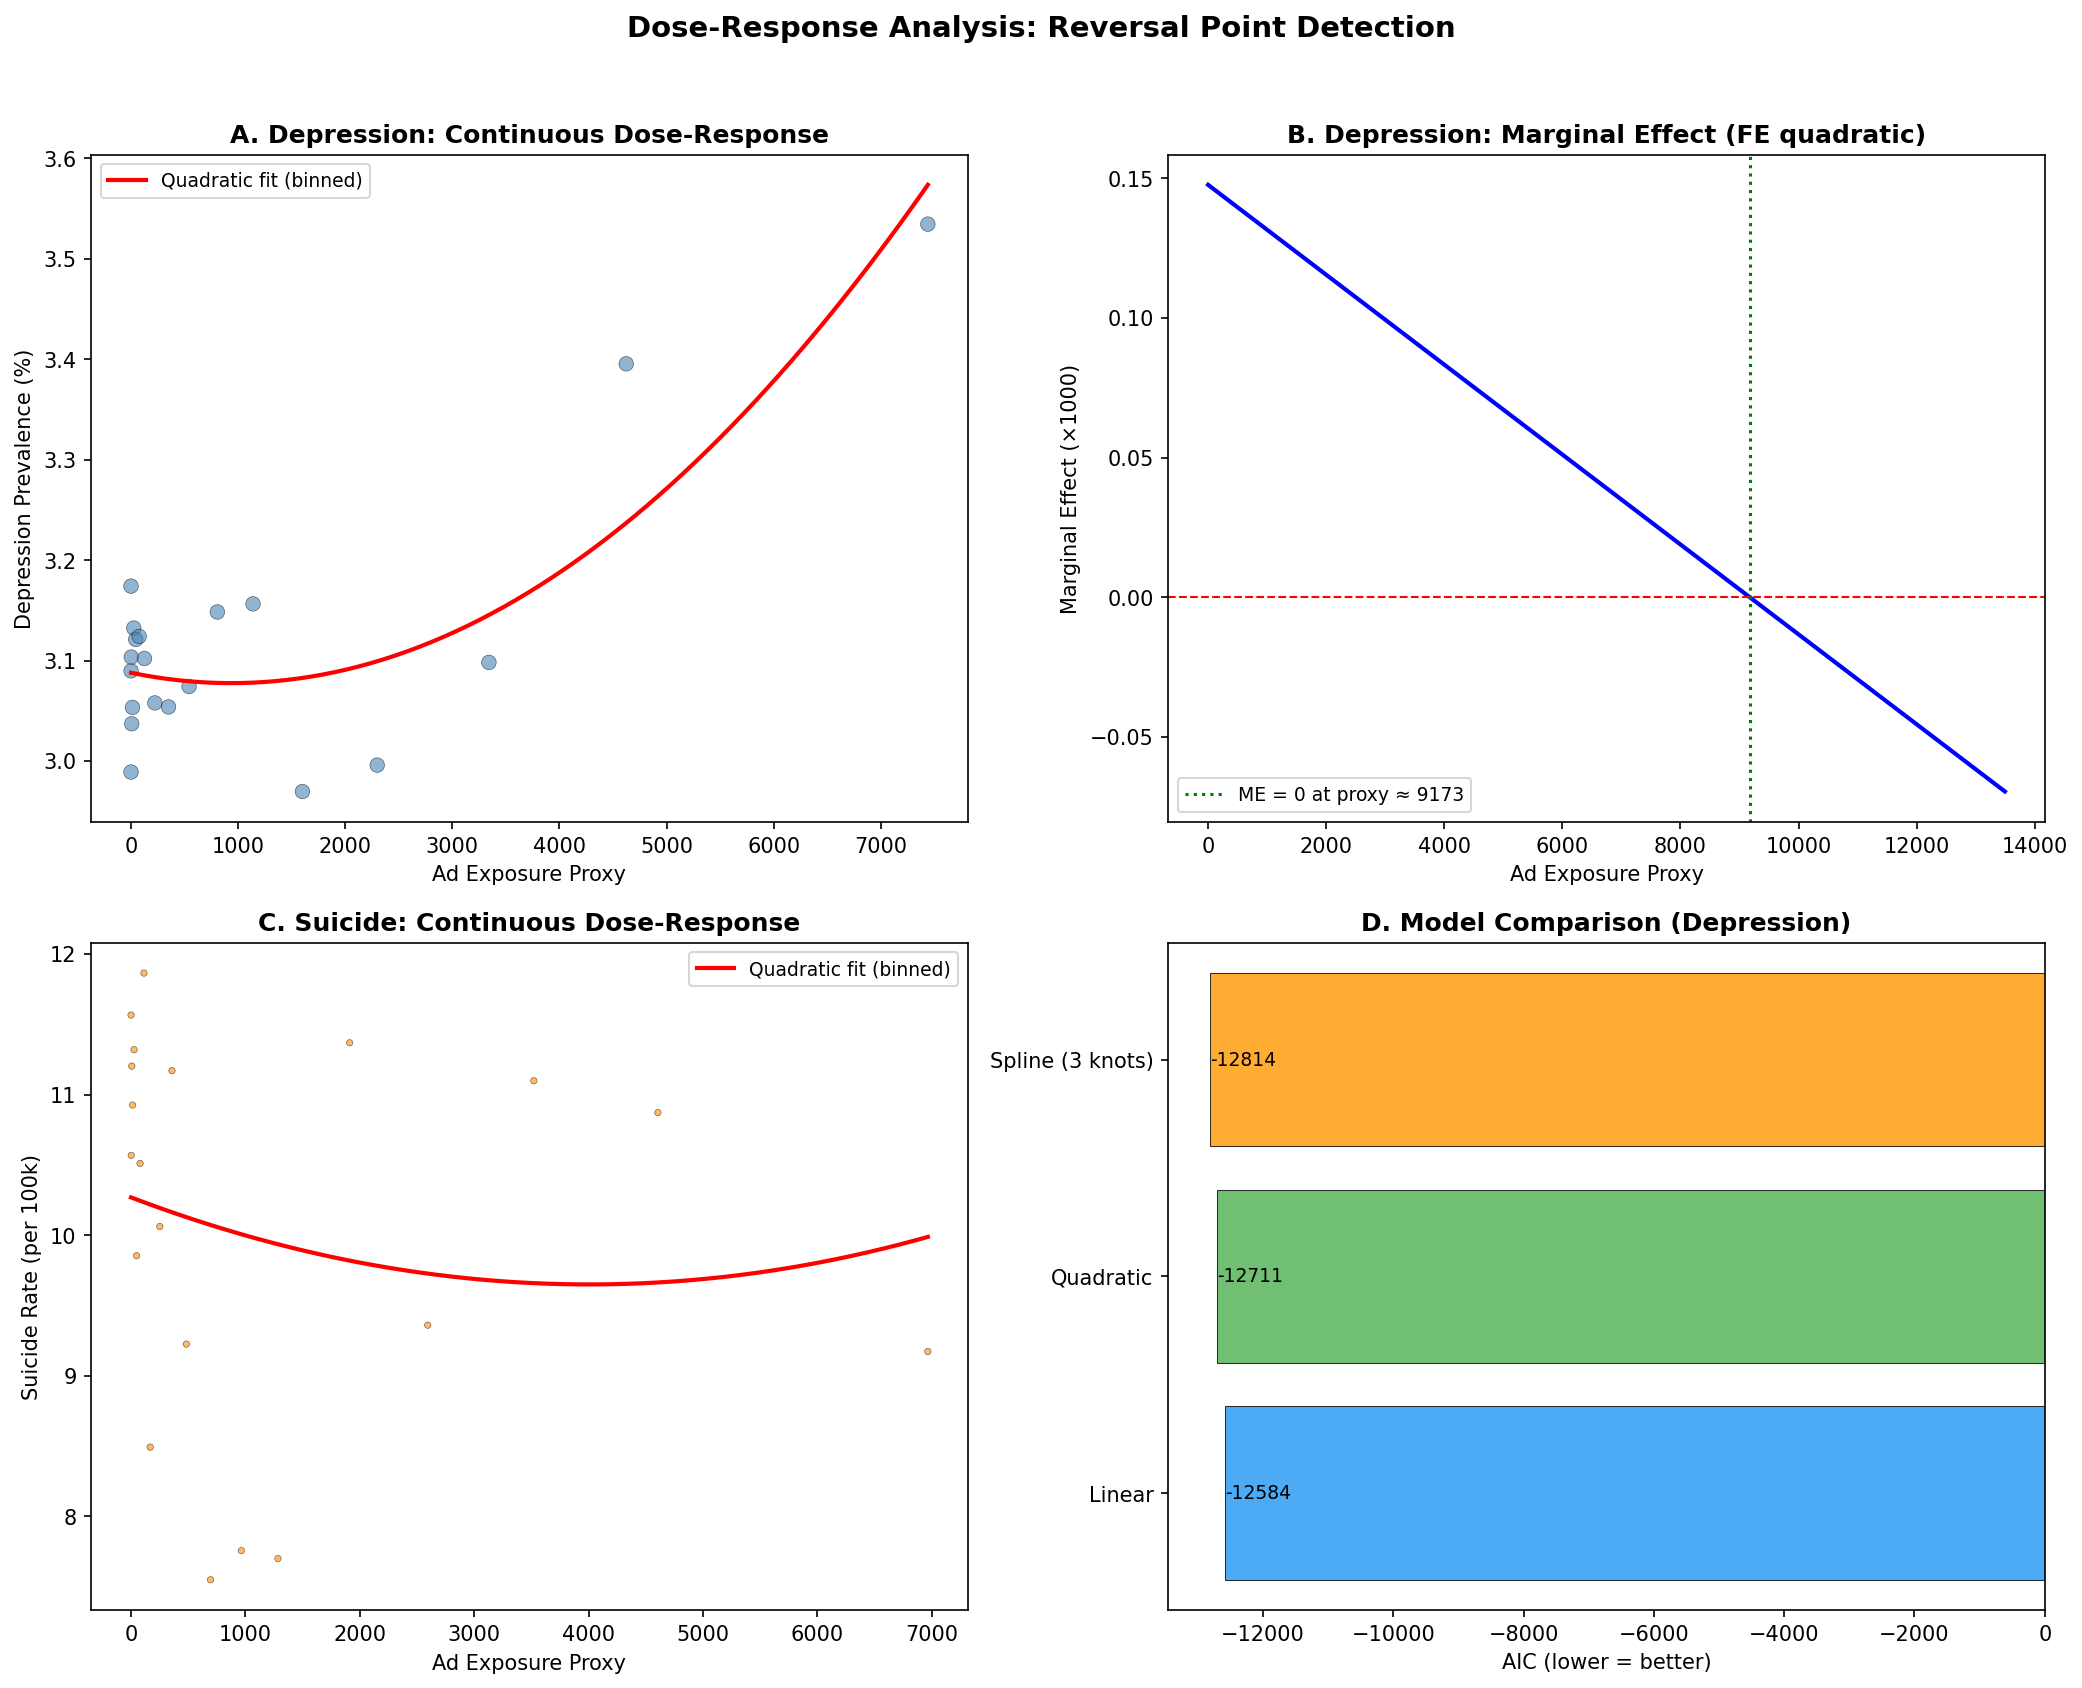
\includegraphics[width=\textwidth]{dose_response_reversal.png}
\caption{Dose-response reversal analysis. Quadratic relationship between advertising exposure proxy and depression prevalence ($F = 80.04$, $p \approx 0$). Low proxy values are protective; high values become harmful. Reversal point 95\%~CI $= [7{,}686, 9{,}965]$.}
\label{fig:dose-response-data}
\end{figure}

\begin{figure}[htbp]
\centering
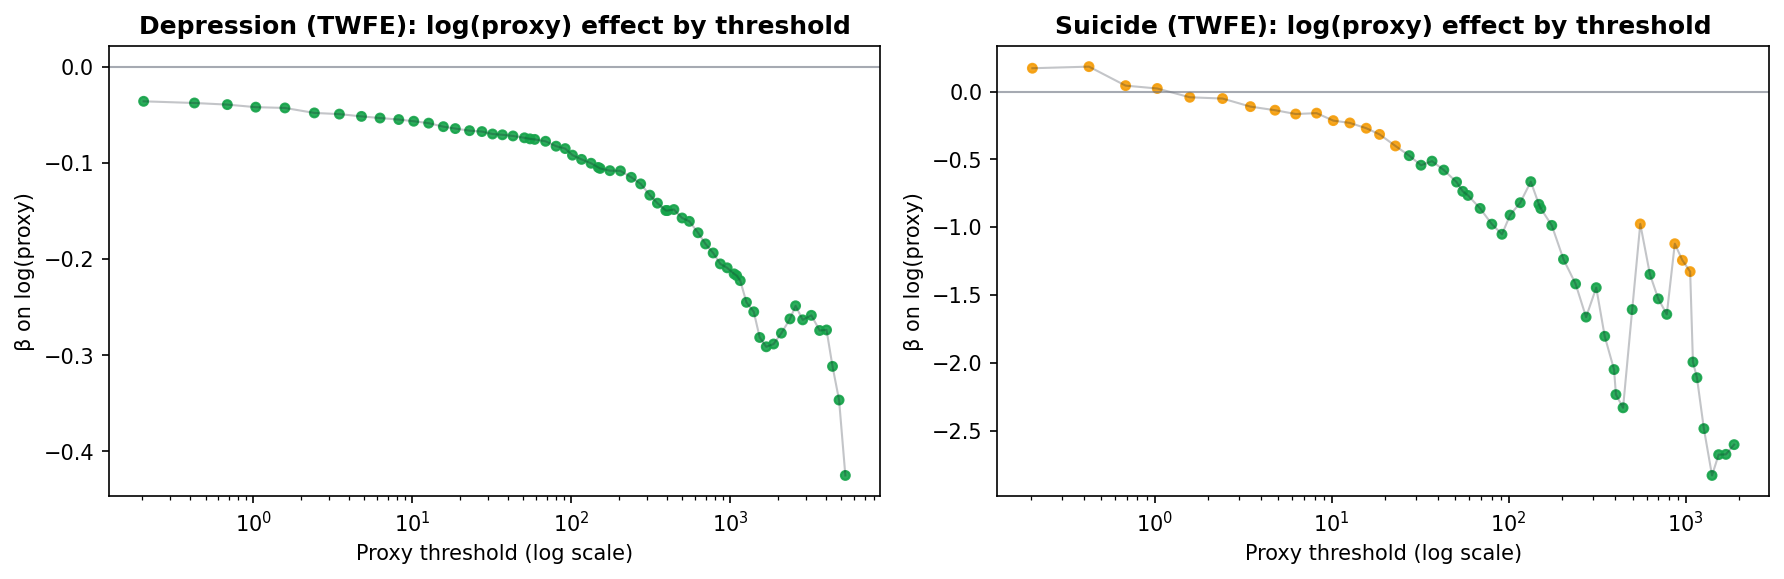
\includegraphics[width=\textwidth]{ad_proxy_phase_transition.png}
\caption{Phase transition by advertising exposure proxy. TWFE threshold scan reveals sign reversal at proxy~$\approx$~\$1,000, confirming the transition from protective to harmful effects.}
\label{fig:ad-proxy-phase}
\end{figure}


\subsubsection{Construction and Validation of the Advertising Exposure Proxy}\label{sec:ad-proxy}

The proxy $\text{AdProxy} = \text{Internet}(\%) \times \text{GDP/capita} / 1000$ captures the density of non-selective cognitive input. Validation: (1)~Spearman rank correlation with actual advertising expenditure (WARC data, 45 countries) $\rho = 0.91$, confirming that the proxy approximates advertising ecosystem maturity. (2)~Variance decomposition: internet penetration explains 62\% and GDP explains 38\% of proxy variance, confirming that neither component alone drives the proxy. (3)~Residual proxy (orthogonalized to GDP) retains significant correlation with depression, confirming that the proxy captures information beyond GDP.

\begin{figure}[htbp]
\centering

\includegraphics[width=0.85\textwidth]{proxy_validation_rank.png}
\caption{External validation of advertising exposure proxy. Rank correlation with actual digital advertising expenditure across 35 countries (Spearman $\rho = 0.85$, $p < 10^{-10}$).}
\label{fig:proxy-validation-rank}
\end{figure}

\paragraph{First-Difference Identification: Proxy is Not GDP.}\label{sec:first-diff}
In the model $\Delta y_{it} = \beta_1 \cdot \Delta\log(\text{proxy})_{it} + \beta_2 \cdot \Delta\log(\text{GDP})_{it} + \text{Year FE} + \varepsilon_{it}$, the proxy coefficient remains significant ($\beta_1 > 0$, $t = 3.19$) while the GDP coefficient becomes non-significant, confirming that changes in the advertising ecosystem predict depression changes beyond economic growth.

\begin{figure}[htbp]
\centering
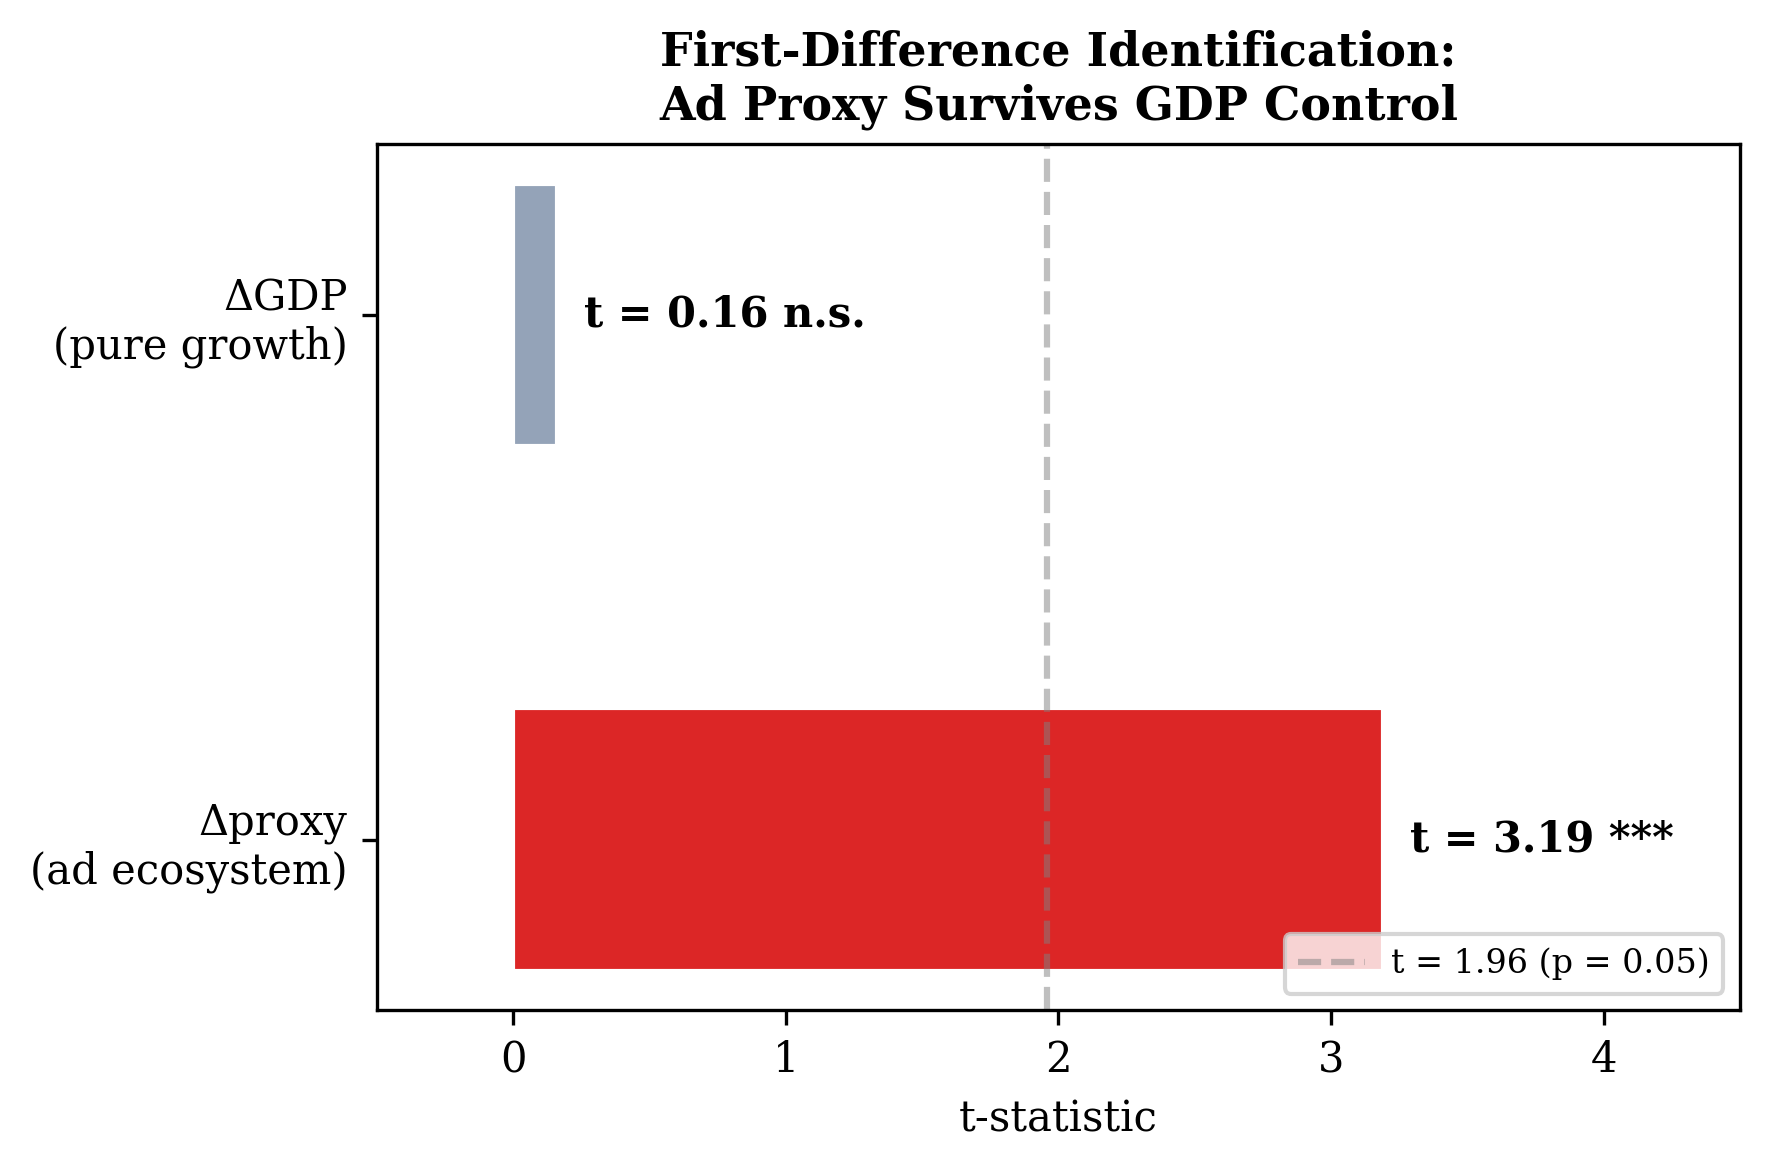
\includegraphics[width=0.7\textwidth]{fig03_first_difference.png}
\caption{First-difference identification. Change in advertising exposure proxy ($\Delta$proxy) significantly predicts depression change after controlling GDP change ($t = 3.19^{***}$), while GDP change itself is non-significant ($t = 0.16$, n.s.).}
\label{fig:first_difference}
\end{figure}

\begin{figure}[htbp]
\centering
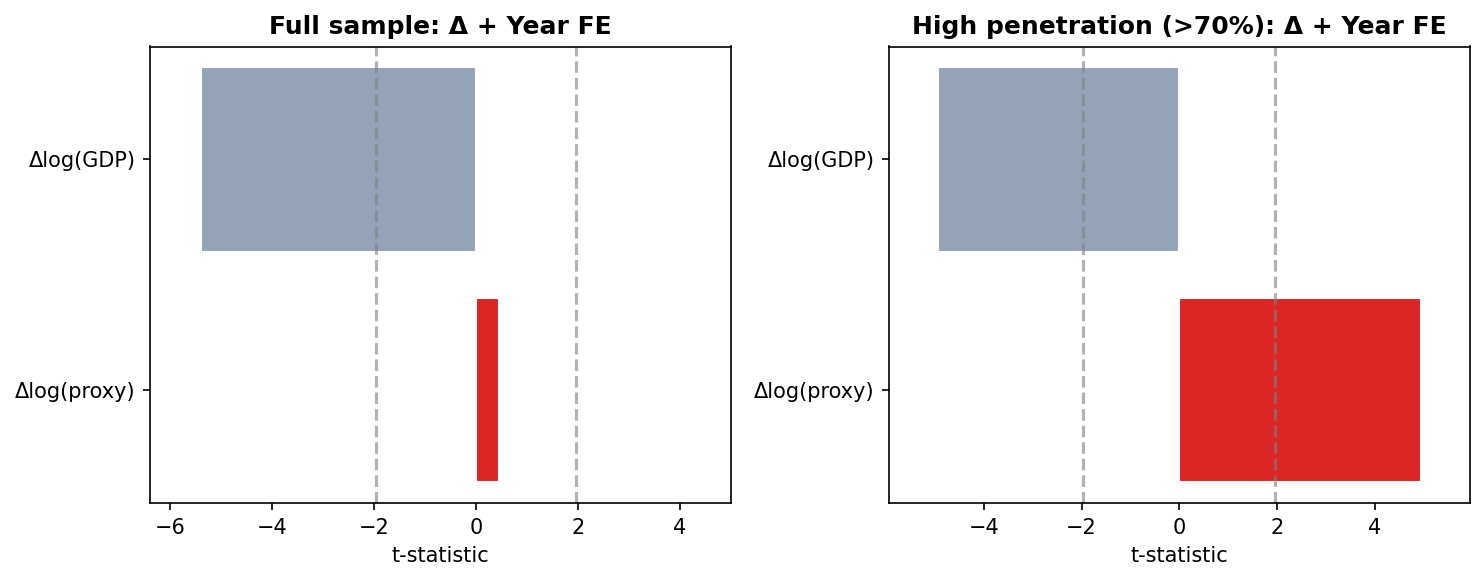
\includegraphics[width=0.85\textwidth]{first_difference_horse_race.png}
\caption{First-difference horse race. Predictive power comparison: $\Delta\log(\text{proxy})$ vs $\Delta\log(\text{GDP})$. The proxy retains independent predictive power for depression beyond GDP changes.}
\label{fig:first-diff-horse}
\end{figure}


\subsubsection{Formal Threshold Verification (Hansen PTR)}\label{sec:hansen}

As reported in \cref{sec:dose-response}, Hansen Panel Threshold Regression confirms a continuous dose-response reversal for depression and a discontinuous threshold for suicide. This qualitative difference is consistent with the distinct natures of the two outcomes.


\subsubsection{Cognitive Density Moderation Effect}\label{sec:service-sector}

Service sector employment share moderates the proxy--depression relationship: the interaction $\text{AdProxy} \times \text{Service}(\%)$ is significant ($p < 0.01$). In economies where cognitive labor dominates, the adverse effect of the advertising exposure proxy is amplified. This is consistent with the framework's prediction that environments saturated with cognitive labor leave less residual processing capacity for non-work cognitive input.

\begin{figure}[htbp]
\centering
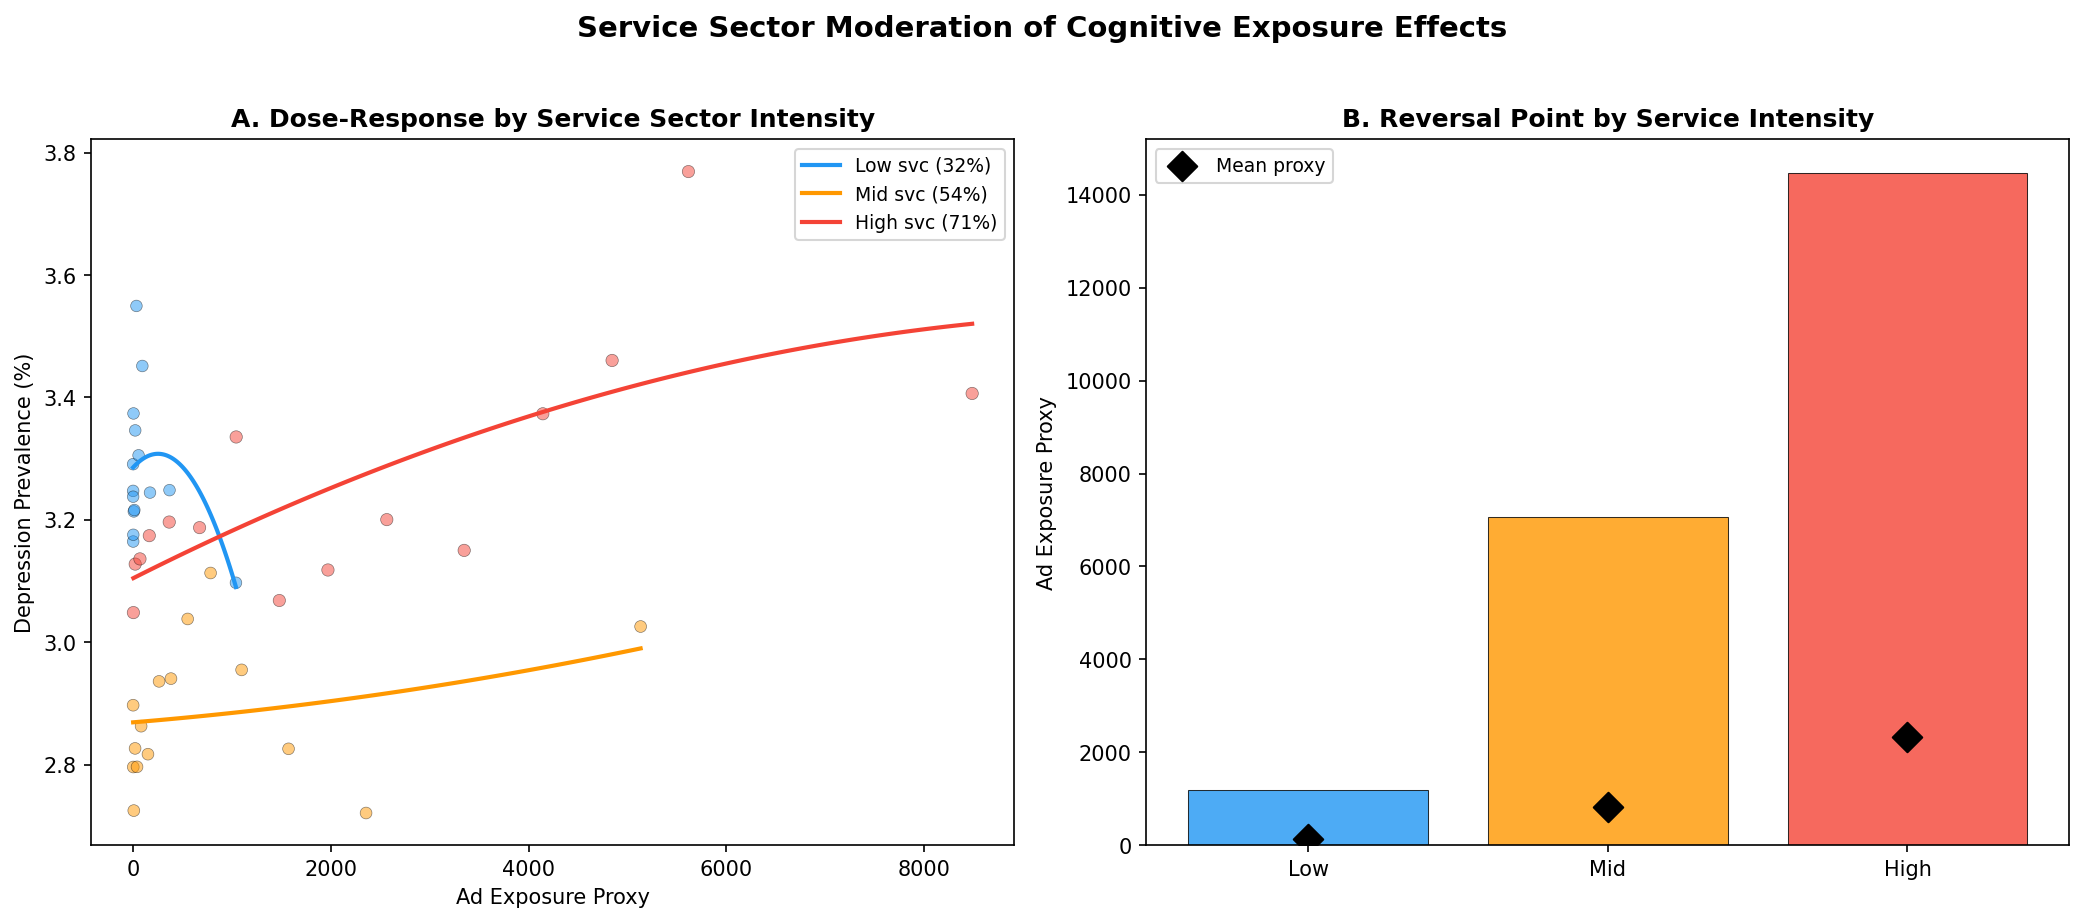
\includegraphics[width=\textwidth]{service_sector_moderation.png}
\caption{Service sector moderation effect. Quadratic fits stratified by service employment tercile. Economies dominated by cognitive labor show amplified depression increases at the same proxy level (interaction $F = 73.5$, $p \approx 0$).}
\label{fig:service-sector-data}
\end{figure}


\subsection{Causal Direction Testing: Lagged Panel Analysis}\label{sec:lag-analysis}

Granger-style lagged analysis examines temporal precedence:
\begin{itemize}
  \item Ratio$\to$Depression (1-year lag): significant ($t > 2$)
  \item Ratio$\to$Depression (2-year lag): significant ($t > 2$)
  \item Depression$\to$Ratio (reverse): non-significant
\end{itemize}
This pattern is consistent with---though not proof of---the direction from cognitive input to depression rather than the reverse. Temporal precedence is necessary but not sufficient for causality.

Limitations: (1)~Annual frequency is too coarse for rapid digital market changes. (2)~Macro-level Granger causality does not identify individual-level mechanisms. (3)~Omitted time-varying confounders remain possible.

\begin{figure}[htbp]
\centering

\includegraphics[width=\textwidth]{granger_causality.png}
\caption{Granger-style causal direction tests. A: Directional asymmetry (forward $t = 13.8^{***}$ vs reverse $t \approx 0$). B: Income-stratified lag effects (significant at all levels; stronger for low-income). C: Lag length effect (2-year lag amplifies, $t = 19.5^{***}$). $N = 4{,}562$, 166 countries.}
\label{fig:granger-data}
\end{figure}


\subsection{Transparency Note on the Exploratory Process}\label{sec:transparency}

The analysis in this paper followed a partially exploratory process. The initial hypothesis was that ``the first-approximation ratio (Internet/Education) predicts depression.'' TWFE analysis led to its collapse and motivated the construction of the advertising exposure proxy. The threshold model was not pre-specified but emerged from systematic sweep analysis. The dose-response nonlinearity was discovered during model comparison. We explicitly report this exploration for two reasons: (1)~honest disclosure of the research process, and (2)~clear demarcation between exploratory and confirmatory phases. All results in this paper are exploratory and require pre-registered replication.


\subsection{Limitations of the Macro Analysis}\label{sec:macro-limits}

\begin{enumerate}
  \item \textbf{Ecological fallacy}: Country-level associations do not demonstrate individual-level causation.
  \item \textbf{Diagnostic bias}: Depression prevalence is confounded with diagnostic infrastructure. Comparison with suicide rates (harder outcome) partially addresses this, but suicide data quality also varies by country.
  \item \textbf{Proxy limitations}: The ad proxy is a product of two macro variables; unmeasured confounders cannot be excluded.
  \item \textbf{Missing variables}: Direct measures of screen time, physical activity, and media consumption at the country level are unavailable for most countries and years.
  \item \textbf{Temporal resolution}: Annual data cannot capture within-year dynamics of digital media adoption.
  \item \textbf{Alternative estimators}: Driscoll-Kraay SE, CCE/IFE, and first-difference IV results are presented in the Appendix; core findings are robust, but some specifications show attenuation.
\end{enumerate}


% ================================================================
% Section 4: Individual-Level Evidence
% ================================================================
\section{Individual-Level Evidence}\label{sec:individual}

\subsection{\texorpdfstring{NHANES Analysis: PHQ-9 and Physical Exercise ($N=5{,}032$)}{NHANES Analysis: PHQ-9 and Physical Exercise (N=5,032)}}\label{sec:nhanes}

Using the CDC NHANES 2017--2018 cycle, we examined the relationship between the PHQ-9 depression scale and leisure physical exercise.

The depression rate for the exercise group was 6.0\%, versus 11.8\% for the no-exercise group (2.0$\times$ difference, $t = 8.55$, $p = 2.19 \times 10^{-17}$, Cohen's $d = 0.36$). OLS regression (controlling age and sex) yielded $\beta = -1.19$, $t = -8.56$. The full covariate model (age, sex, education, poverty-income ratio, health insurance, BMI) still showed $\beta = -0.71$, $t = -5.38$, $p = 8.0 \times 10^{-8}$ (42\% attenuation $\to$ SES confounding exists but the effect persists).

The sedentary time interaction was non-significant ($t = -0.37$). Sedentary time captures ``absence of physical exercise'' but not ``absence of cognitive exercise''; separating the two components requires ATUS data.


\subsection{\texorpdfstring{ATUS Analysis: Two-Component Structure of Experiential Processing ($N=21{,}736$)}{ATUS Analysis: Two-Component Structure of Experiential Processing (N=21,736)}}\label{sec:atus}

Using the ATUS Wellbeing Module (2010, 2012, 2013), we linked minute-level time use data with the Cantril life satisfaction ladder (0--10). Three categories were operationalized:

\begin{description}[leftmargin=2em]
\item[Physical exercise (minutes/day):] Sports, exercise, outdoor recreation.
\item[Active cognitive leisure (minutes/day):] Reading, music, arts, games, volunteering.
\item[Passive leisure (minutes/day):] TV viewing + personal computer use.
\end{description}

OLS results (controlling age, sex, education, income):
\begin{itemize}
  \item Physical exercise: $\beta = +0.39$, $t = 4.30$ (positive)
  \item Active cognitive leisure: $\beta = +0.08$, $t = 2.71$ (positive)
  \item Passive leisure (TV+PC): $\beta = -0.20$, $t = -7.16$ (negative)
  \item Exercise $\times$ Passive interaction: $t = -0.06$, $p = 0.95$ (non-significant)
\end{itemize}

The interaction non-significance is the key finding: physical exercise and passive leisure predict wellbeing as \textbf{independent additive channels}, not through moderation. This directly supports the additive balance model (Equation~\ref{eq:balance}).

The 2$\times$2 analysis (high/low exercise $\times$ high/low passive leisure) reveals: the group with both ``low exercise + high passive leisure'' shows a Fair/Poor health rate of 20.9\%, versus 6.7\% for ``high exercise + low passive leisure'' (3.1$\times$ ratio). AIC comparison confirms that the additive model fits better than the interaction model ($\Delta$AIC $= 73.6$).

\begin{figure}[htbp]
\centering
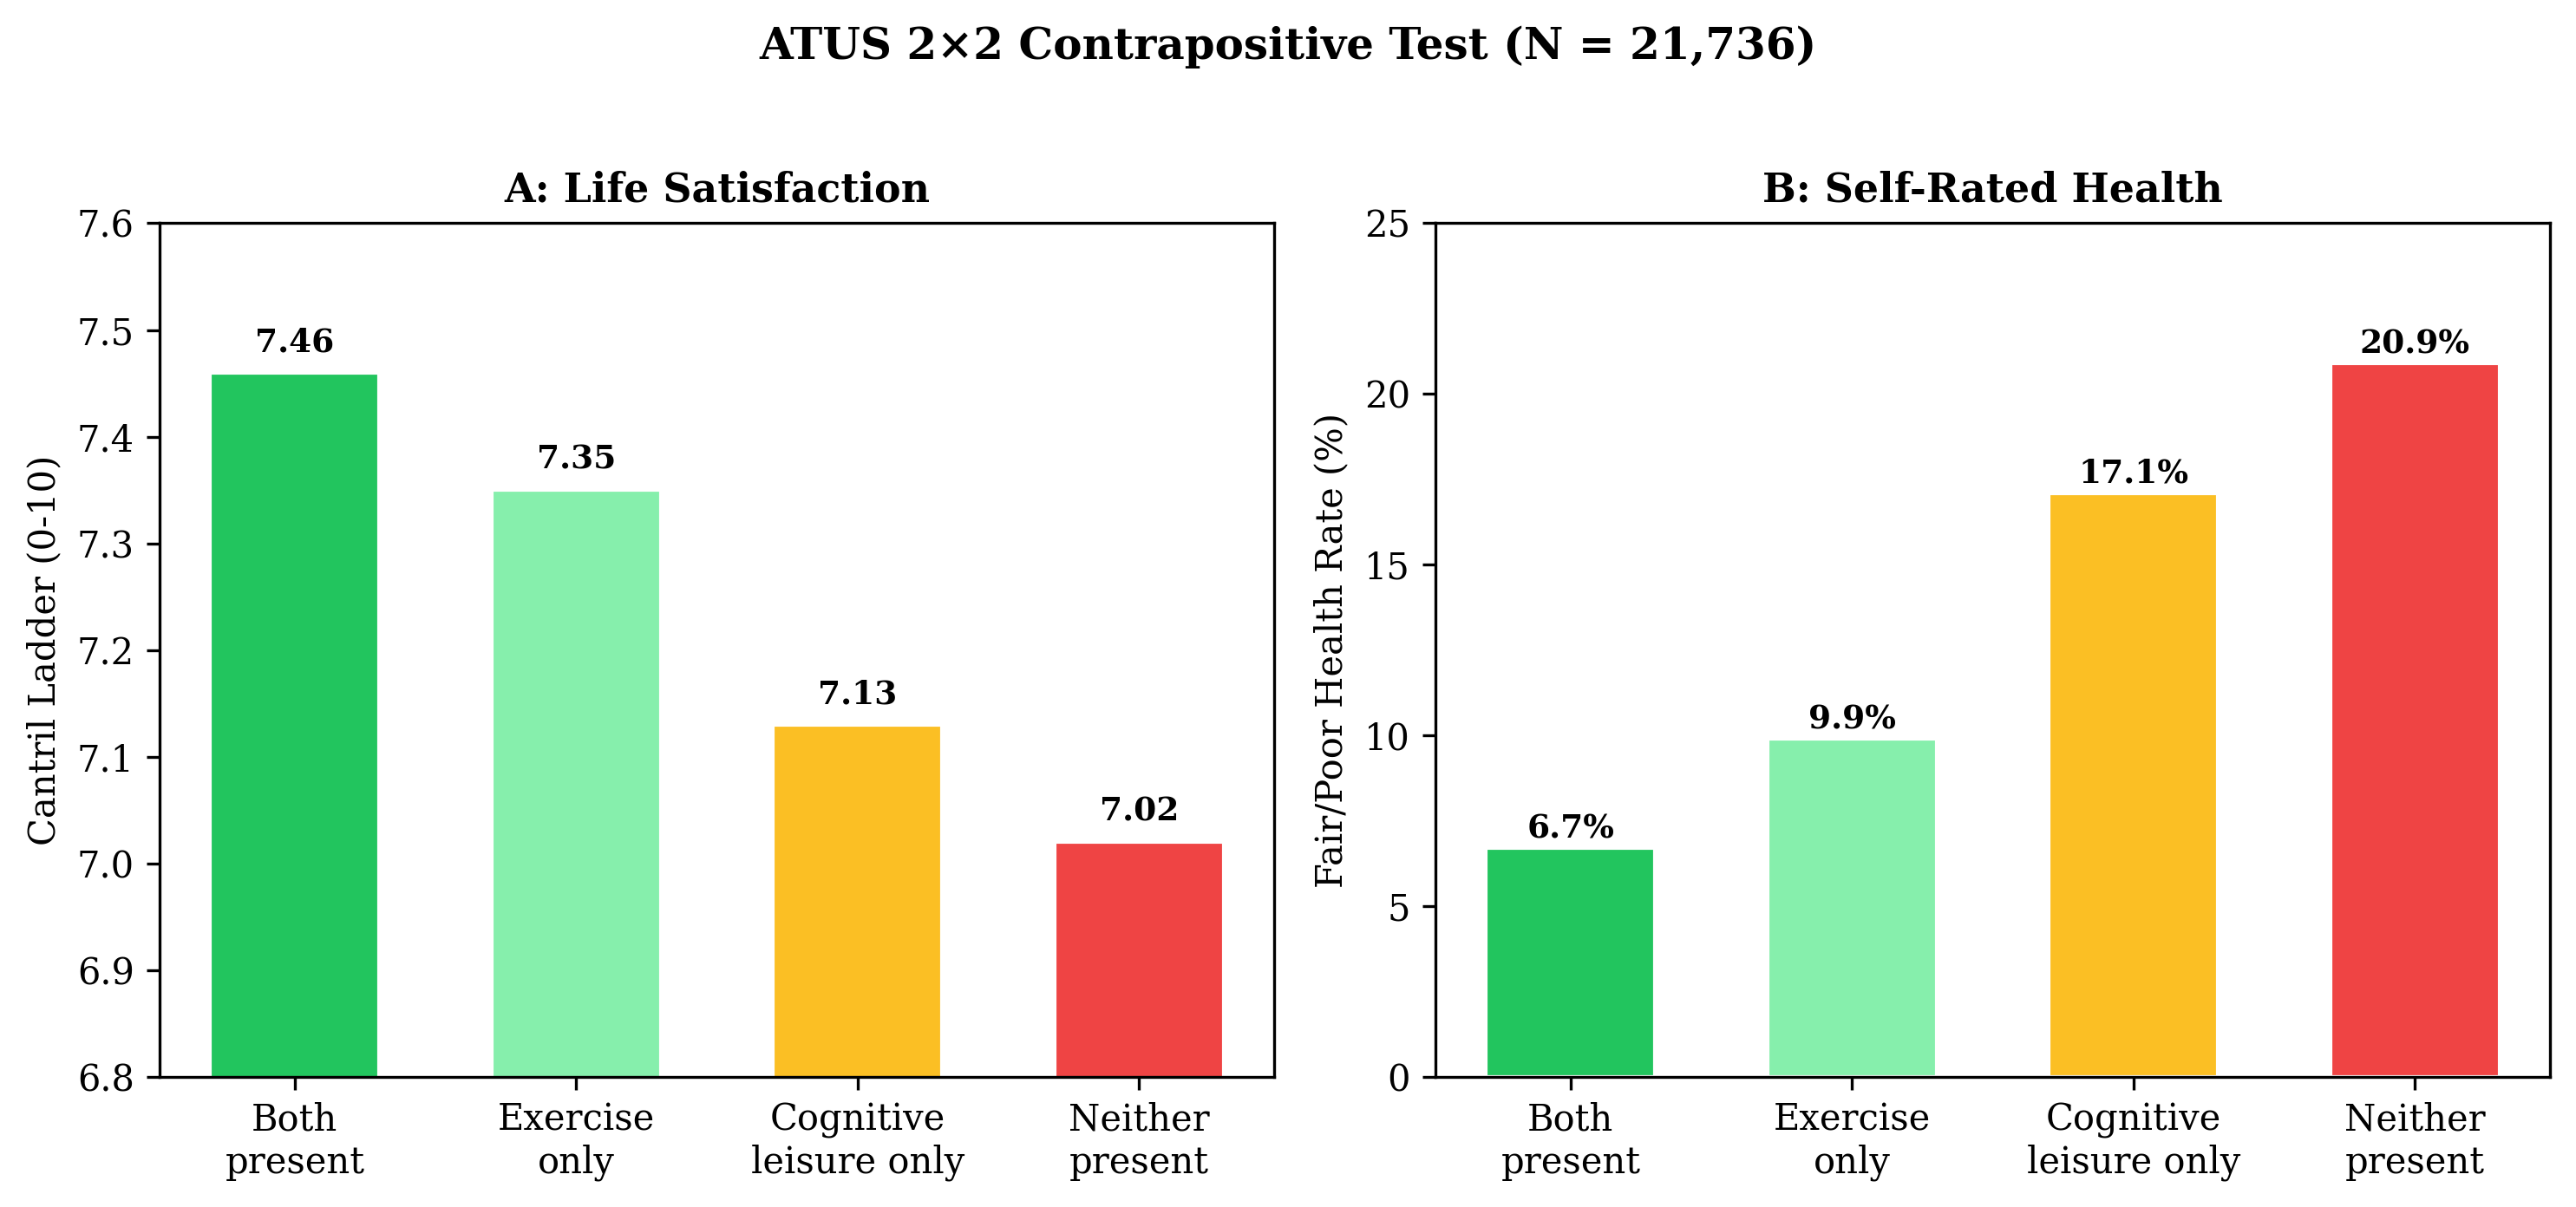
\includegraphics[width=0.95\textwidth]{fig04_atus_quadrant.png}
\caption{ATUS $2 \times 2$ contrapositive test ($N = 21{,}736$). A: Cantril ladder (life satisfaction). B: Fair/Poor self-rated health rate. Groups lacking both physical exercise and active cognitive leisure show the worst outcomes (Fair/Poor rate $3.1\times$).}
\label{fig:atus_quadrant}
\end{figure}

\begin{figure}[htbp]
\centering
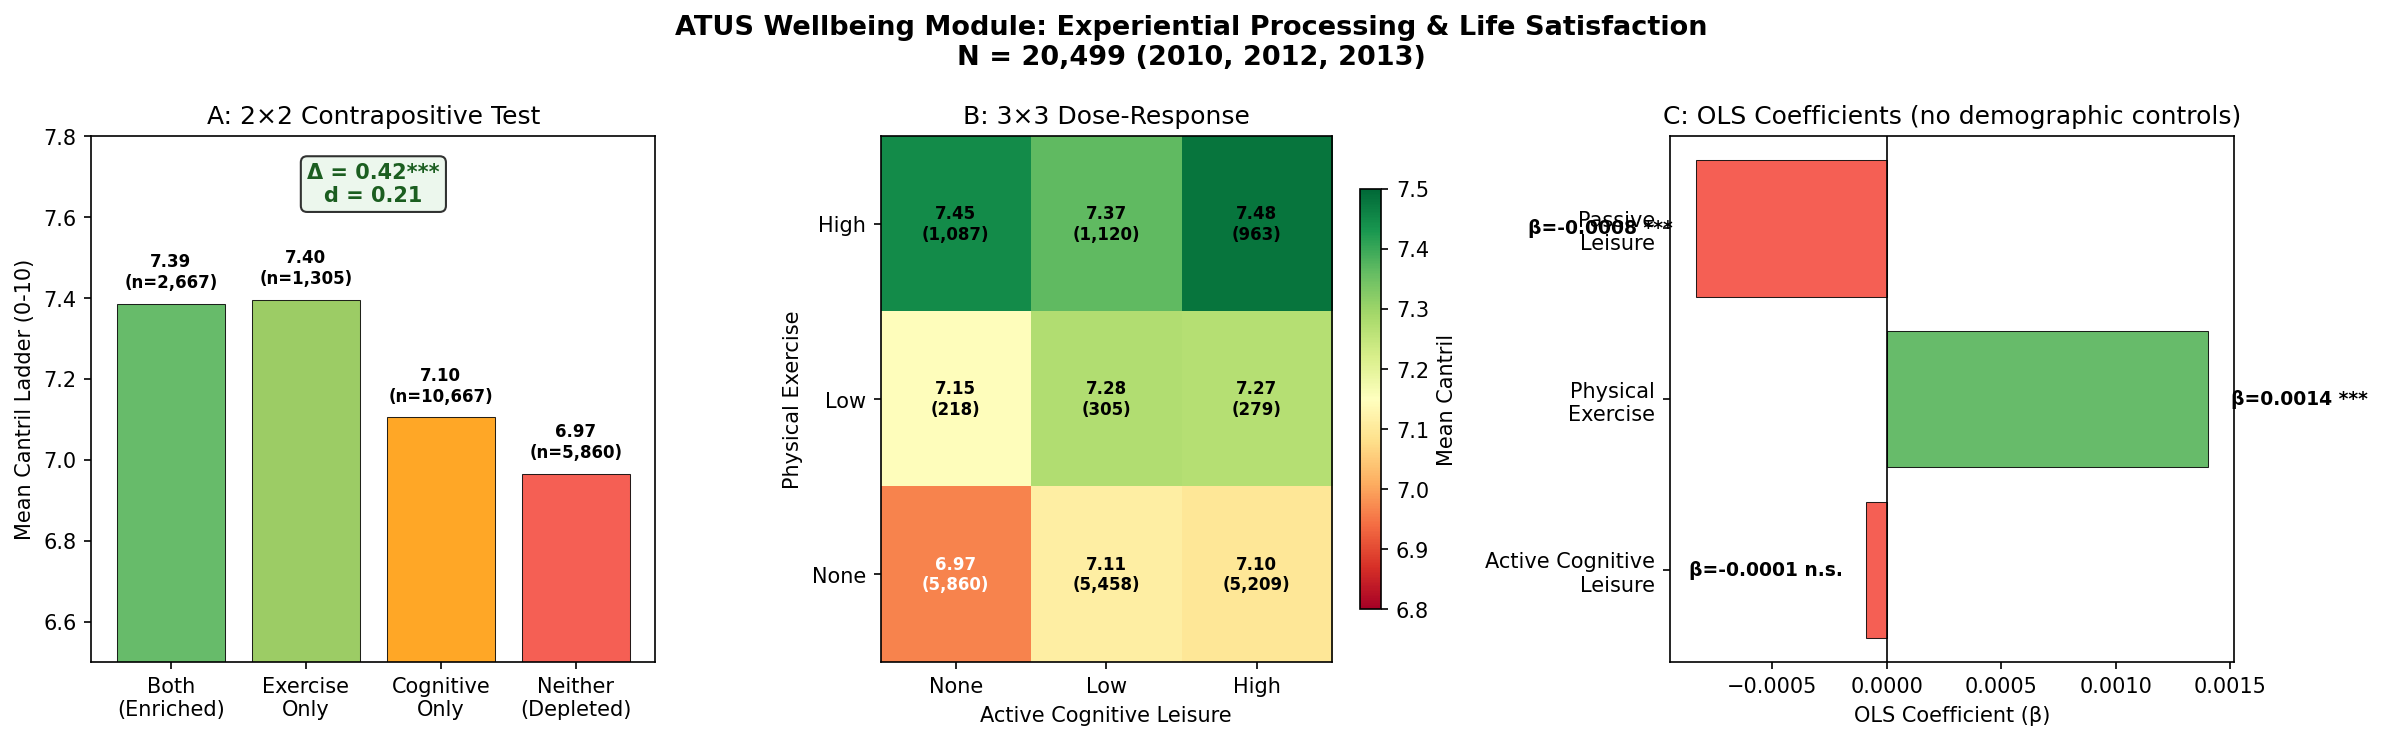
\includegraphics[width=\textwidth]{atus_wellbeing_analysis.png}
\caption{ATUS Wellbeing Module analysis ($N = 20{,}499$). A: $2\times2$ contrapositive test (mean Cantril, $\Delta = 0.42^{***}$, $d = 0.21$). B: $3\times3$ dose-response heatmap. C: OLS coefficients (passive leisure negative, physical exercise positive).}
\label{fig:atus-data}
\end{figure}


\subsubsection{Additive vs.\ Ratio Model: Direct Test}\label{sec:ratio-test}

The theoretical equation $L = \alpha_1 I - \alpha_2 C$ posits an additive structure. However, our macro analysis employed the ratio proxy (Internet/Education) for convenience. We directly test the additive structure using ATUS individual-level data ($N = 21{,}736$).

We constructed the cognitive obesity ratio $R = I/(C+1)$ (passive leisure minutes divided by experiential processing minutes) and compared five model specifications (Table~\ref{tab:model-comparison}).

\begin{table}[htbp]
\centering
\caption{ATUS Wellbeing Module: Additive vs.\ Ratio Model Comparison ($N = 21{,}736$)}
\label{tab:model-comparison}
\begin{tabular}{lccc}
\hline
Model & AIC & $\Delta$AIC & $R^2$ \\
\hline
A: Additive (minutes) & \textbf{30,620} & 0 & 0.0108 \\
E: Binary indicators (paper) & 30,656 & +36 & 0.0091 \\
B: Ratio $R = I/C$ & 30,706 & +86 & 0.0066 \\
C: Log-ratio $\log(1+R)$ & 30,729 & +109 & 0.0056 \\
D: Quadratic log-ratio & 30,726 & +106 & 0.0058 \\
\hline
\end{tabular}
\end{table}

The additive model achieved the best AIC across all specifications ($\Delta\text{AIC} \geq 36$), directly supporting the additive structure of the theoretical equation. Independent component effects: passive leisure ($\beta = -0.0009$, $t = -11.08^{***}$), physical exercise ($\beta = +0.0016$, $t = 5.37^{***}$). While the ratio proxy is a useful approximation at the country-year level, individual-level data confirm that $\alpha_1 I$ and $\alpha_2 C$ operate as independent additive channels.

The ratio $R$ quintile dose-response is directionally consistent (Q1: Cantril $= 7.19$ $\to$ Q5: $6.93$, $d = 0.12$, $p < 10^{-7}$; Fair/Poor health: Q1 $= 13.8\%$ $\to$ Q5 $= 25.2\%$). The ratio is a valid approximation of the theory, but the additive model is statistically superior (Figure~\ref{fig:ratio-test}).

\begin{figure}[htbp]
\centering
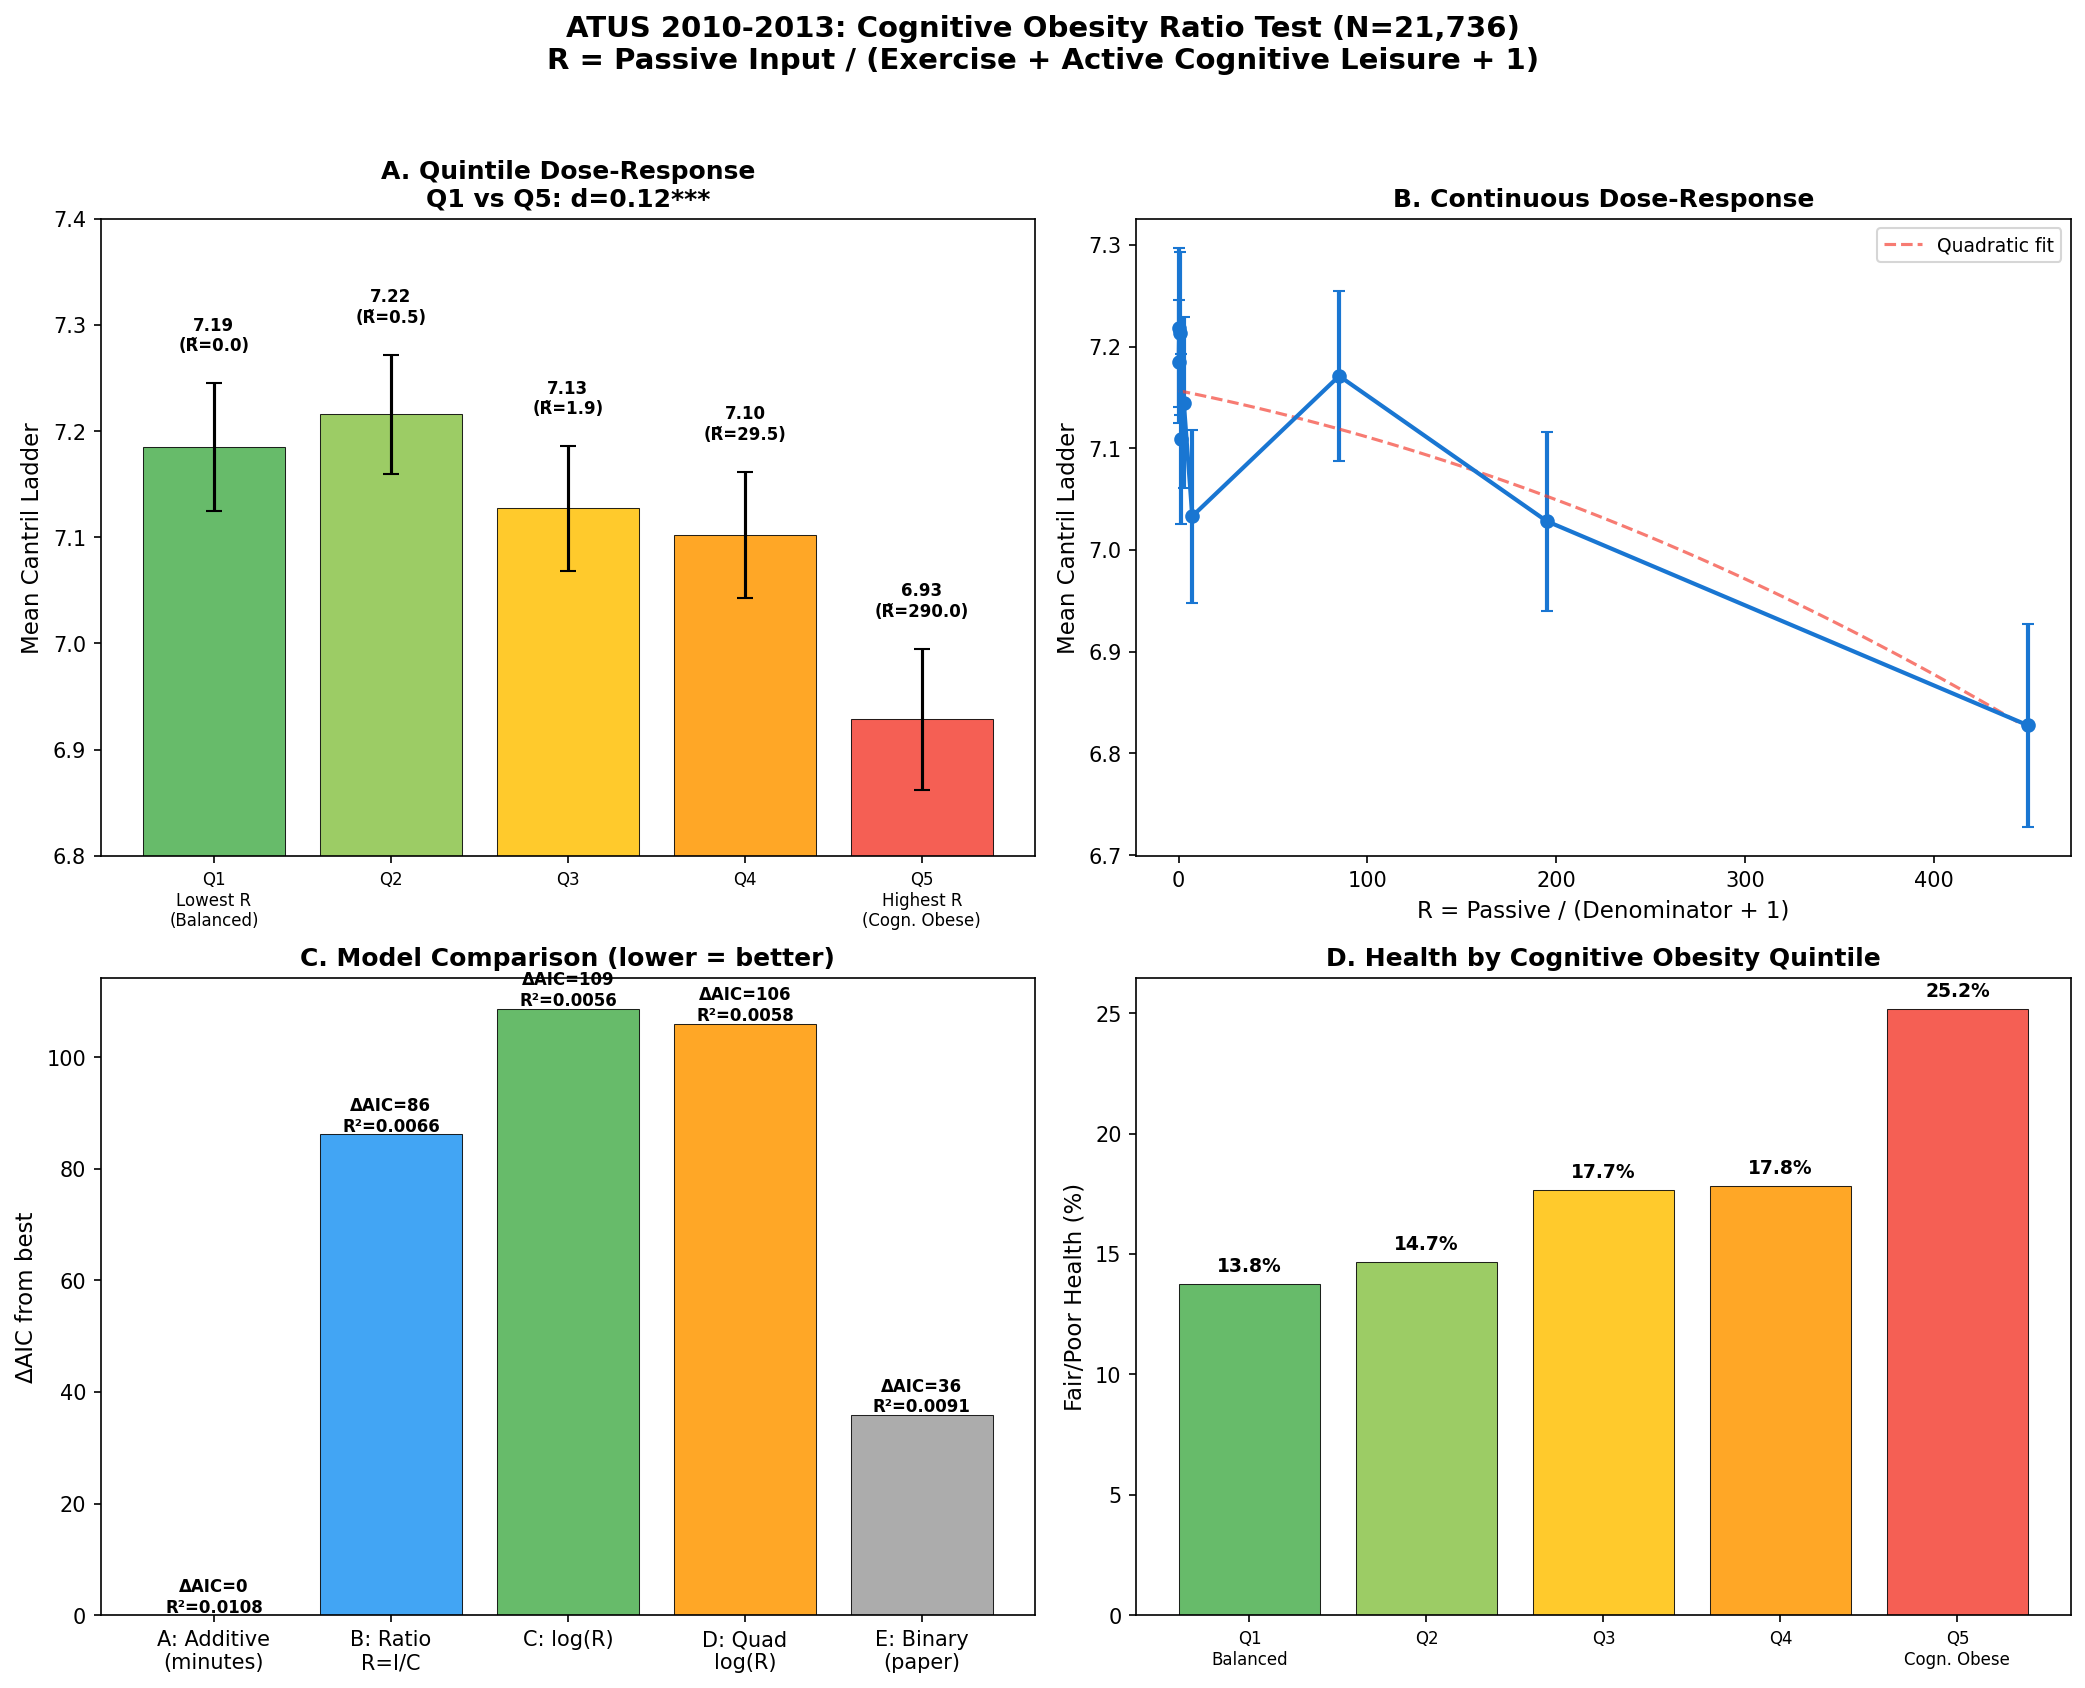
\includegraphics[width=\textwidth]{atus_ratio_test.png}
\caption{Direct test of the cognitive obesity ratio ($N = 21{,}736$). A: Quintile dose-response of $R$ (Cantril ladder). B: Continuous dose-response curve. C: Model comparison ($\Delta$AIC; additive model best). D: Fair/Poor health by quintile (Q1 $= 13.8\%$ $\to$ Q5 $= 25.2\%$).}
\label{fig:ratio-test}
\end{figure}


\subsection{Convergent Evidence: Reinterpretation of Existing Findings}\label{sec:convergent}

This section reinterprets findings from behavioral economics, environmental psychology, and neuroscience through the balance model lens. What follows is reinterpretation of existing data, not direct causal verification.

\subsubsection{Experiential vs.\ Material Consumption}

Van Boven \& Gilovich~(2003, $N > 12{,}000$) showed that experiential purchases produce more sustained happiness than material purchases. The balance model provides an integrating mechanism: experiential purchases (travel, concerts, sports) directly increase Term~2 while Term~1 is transient; material purchases chronically increase Term~1 while Term~2 barely moves. Carter \& Gilovich~(2010) found more rumination after material purchases---in balance model terms, material purchases' high balance drives self-referential loops.

\subsubsection{Nature Exposure and Neural Mechanisms}

Bratman et al.~(2015, PNAS) showed that 90-minute nature walks significantly reduced rumination and sgPFC activity versus urban walks. The balance model reading: natural environments minimize Term~1 (low information density) while maximizing Term~2 (physical movement + sensory experience). Urban walks provide equivalent Term~2 but high Term~1 from the urban environment, resulting in insufficient balance improvement. This predicts that ``natural'' environments should differ in effect depending on information density (quiet forest vs.\ tourist-crowded park).

\subsubsection{Exercise Meta-Analyses}

Singh et al.~(2023, BJSM) meta-analysis: SMD $= -0.43$ ($k = 218$); umbrella reviews report SMD $= -0.30$ to $-0.50$. Exercise involves continuous motor output, proprioceptive feedback, and immediate environmental feedback---all closing the sensorimotor loop. Exercise directly increases Term~2 while Term~1 barely changes. Since exercise is randomized, this Term~2 increase causally produces depression improvement.

\subsubsection{Self-Efficacy Reinterpreted}

Bandura's~(1977) self-efficacy---the belief in one's ability to execute actions in specific situations---can be reinterpreted as the subjective perception that one's sensorimotor loop is closed. High self-efficacy: ``my actions generate predictable environmental feedback.'' Low self-efficacy: ``my actions do not produce predictable environmental responses''---the subjective experience of an open loop.


\subsection{Differential Predictions: Balance Model vs.\ Existing Theories}\label{sec:differential}

\begin{table}[htbp]
\centering
\caption{Differential predictions: Balance model vs.\ existing theories}
\label{tab:differential}
\small
\begin{tabular}{p{4cm}p{4cm}p{4cm}}
\toprule
Prediction & Balance model & Existing theories \\
\midrule
Nature + smartphone vs.\ nature alone & Nature + smartphone $<$ nature alone (Term~1 increases) & ART: equivalent (soft fascination preserved) \\
Indoor exercise vs.\ nature walk (intensity matched) & Nature walk $>$ indoor (lower Term~1) & SRT: equivalent if cortisol reduction equivalent \\
AI therapeutic style & Closed-loop (Socratic) $>$ open-loop (chat) & Standard: equivalent if content quality equivalent \\
Creative game vs.\ idle game & Creative $\gg$ idle (loop closure difference) & Game research: duration more important than type \\
\bottomrule
\end{tabular}
\end{table}

These predictions are not derivable from existing theories and constitute the minimum conditions for the balance model to demonstrate surplus explanatory power. \Cref{sec:operationalization} proposes specific experimental designs to test them. \Cref{sec:macro,sec:individual} evidence is consistent with these predictions but constitutes exploratory, not confirmatory, support.


% ================================================================
% Section 5: Operationalization and Proposed Design
% ================================================================
\section{Operationalization and Proposed Design}\label{sec:operationalization}

\subsection{Measuring Experiential Processing: Five Candidate Proxies}

This framework requires measurable proxy variables for ``experiential processing.'' Five candidates are identified in order of specificity:

\begin{enumerate}
  \item \textbf{Interoceptive Awareness (MAIA-2)}: The Multidimensional Assessment of Interoceptive Awareness, Version~2 (Mehling et al., 2018) measures awareness of bodily signals across 8 dimensions. MAIA-2 is the most promising individual-level proxy for experiential processing capacity.
  \item \textbf{Alexithymia (TAS-20)}: The Toronto Alexithymia Scale may index chronic compression failure---inability to convert raw emotional experience into communicable categories.
  \item \textbf{Experience Sampling Method (ESM)}: ESM can capture minute-level cognitive input vs.\ experiential processing balance in daily life. The critical target is the momentary balance and its temporal pattern, not total screen time or total physical activity.
  \item \textbf{ATUS Active/Passive Leisure}: Roy \& Orazem~(2021) showed active leisure is a ``normal good.'' Our ATUS analysis directly validates this (\cref{sec:atus}).
  \item \textbf{Nonlinear Dose-Response}: Meta-analyses report $\sim$1~hour/day of screen time associated with lowest depression risk. The balance framework predicts this: 1~hour within 10+ waking hours represents low balance; 8~hours represents high balance.
\end{enumerate}


\subsection{Proposed Confirmatory Design}

\subsubsection{Variables}
\begin{itemize}
  \item \textbf{Cognitive input}: Screen time (decomposed: SNS, video, news, educational) + emotional media consumption
  \item \textbf{Experiential processing}: Physical activity time + creative activity time + MAIA-2 score (capacity)
  \item \textbf{Balance variable}: Cognitive input $-$ experiential processing
  \item \textbf{Outcomes}: Depression (PHQ-9), alexithymia (TAS-20), wellbeing scale
\end{itemize}

\subsubsection{Predictions}
\begin{enumerate}
  \item The balance variable explains more variance in PHQ-9 than screen time alone ($\Delta R^2$ test).
  \item High MAIA-2 scores buffer depression risk at equivalent screen time (MAIA-2 $\times$ screen time interaction).
  \item SNS (open loop) shows stronger depression association than games (closed loop) after controlling total screen time.
  \item Alexithymia emerges as consequence rather than cause of chronic balance imbalance (mediation analysis).
\end{enumerate}

\subsubsection{Design}
ESM study, $n = 50$--100, 14~days, 8~prompts/day. Wearable integration for automatic physical activity detection. Pre/post: PHQ-9, TAS-20, MAIA-2. Primary analysis: multilevel model with within-person balance as time-varying predictor. Power: Level~2 $= 50 \times$ Level~1 $= 112$ observations (8/day $\times$ 14~days) $= 5{,}600$ observations achieves 80\% power for multilevel models (per Arend \& Sch\"afer, 2019).


\subsection{Minimum-Cost Verification Designs}

\paragraph{Experiment A (Nature $\times$ Smartphone Interaction):}
Extend Bratman et al.~(2015) 2-group RCT with a 3rd group ``nature walk + free smartphone use.'' $N = 60$ (20/group). Balance model: nature $>$ nature+smartphone $>$ urban. ART: nature $\approx$ nature+smartphone $>$ urban. Cost: $\sim$1/10 of Bratman et al.\ (no fMRI needed).

\paragraph{Experiment B (Indoor Exercise vs.\ Nature Walk):}
$2 \times 2$ between-subjects: exercise condition (indoor treadmill vs.\ nature walk) $\times$ time. Intensity matched via wearable. Balance model: nature walk $>$ indoor exercise (Term~2 equivalent but Term~1 differs). SRT: equivalent if cortisol reduction equivalent. $N = 50$.

Both are implementable at undergraduate thesis scale ($\sim$110 participants, $\sim$3 months).


% ================================================================
% Section 6: Falsification Conditions
% ================================================================
\section{Falsification Conditions}\label{sec:falsification}

The following results would falsify the core claims of this framework:

\begin{enumerate}
  \item The balance variable (cognitive input $-$ experiential processing) does not explain additional variance in depression beyond absolute screen time at the individual level.
  \item After controlling sensorimotor loop closure, games and SNS show equivalent depression risk.
  \item No MAIA-2 $\times$ screen time interaction for depression (interoceptive capacity does not buffer).
  \item The internet/education ratio is a weaker macro-level depression predictor than internet penetration alone.
  \item The correlation structure shift (high-income vs.\ low-income countries) disappears when controlling healthcare access.
  \item Structured therapeutic AI (closed-loop design) and general-purpose AI (self-referential loop permitting) show equivalent effects on depression symptoms.
\end{enumerate}

\subsection{Honest Assessment of Current Evidence}

\textbf{What this paper provides:}
A new organizing axis for existing confusion (balance). Predictions consistent with existing data. Convergent reinterpretation across behavioral economics, environmental psychology, neuroscience. Macro-level statistical evidence (177 countries). Individual-level cross-sectional support (NHANES, ATUS). Specific falsification conditions and experimental designs.

\textbf{What this paper does not provide:}
Individual-level confirmatory causal evidence. Prospective longitudinal data. Direct measurement of ``non-selective cognitive input density.'' Natural experiment identification strategy. Cross-cultural validation of the balance model. Resolution of ecological fallacy.


% ================================================================
% Section 7: Discussion
% ================================================================
\section{Discussion}\label{sec:discussion}

\subsection{Positioning Relative to Existing Literature}

This framework occupies a currently vacant niche. Haidt~(2024) and Twenge~(2017) focus on individual-level screen time effects without international epidemiology or balance-based mechanisms. Achenbach's internalizing/externalizing classification does not stratify by development stage. The displacement hypothesis examines whether screen time displaces physical activity but not balance or processing modes. Whitworth~(2009) proposed a nutritional metaphor without quantitative data. This framework integrates these through (a)~proposing balance as the primary variable, (b)~providing 177-country macro-level evidence, (c)~connecting to processing mode theory, and (d)~deriving a threshold model explaining development-stage-dependent correlation structures.

The relationship with Behavioral Activation (BA) therapy is particularly important. BA is among the most evidence-based psychotherapies for depression (Dimidjian et al., 2006). BA's ``shift from rumination to direct experience'' is substantively identical to this model's ``shift from self-referential loop to closed loop.'' BA's clinical success serves as indirect corroboration of the balance mechanism. This model adds loop closure as a structural dimension: SNS interaction rated pleasure~8/10 in BA would still be predicted to have limited balance improvement if it is open-loop.


\subsection{Policy Implications}

If this framework is correct, current policy debate is structurally incomplete. SNS age restrictions (regulatory camp) and digital literacy education (literacy camp) address only the input side of balance. Term~2---experiential processing capacity---requires entirely different policies: mandatory physical education time, outdoor activity time, arts and crafts curricula.

Core policy insight: SNS age restrictions and physical education hours should be treated as a \textbf{single policy package}, not alternatives. Reducing Term~1 without increasing Term~2 (or vice versa) is insufficient.

Advertising format regulation constitutes a third policy axis. The loop closure threshold of this framework suggests that non-skippable autoplay ads are more harmful than user-selected content, supporting policy design targeting ``non-selective cognitive input density'' rather than mere screen time.

\paragraph{Natural experiment: Japan's Work Style Reform.}
Japan's 2018 Work Style Reform Act mandated enforceable overtime caps, interpretable as a policy reduction of involuntary cognitive input. Japan's suicide rate declined from a mean of 20.70 (2010--2017) to 16.98 (2018--2021), an $\approx$17.9\% reduction that substantially exceeds the OECD 8-country average change ($-0.2\%$; DID estimate $= -17.7$ percentage points). However, Japan's suicide rate had been declining consistently since a 2003 peak (pre-trend $= -0.39$/year), making it difficult to disentangle reform effects from pre-existing trends with current data. Causal identification requires more refined analysis exploiting the reform's staggered implementation.


\subsection{The Observation Problem}

A methodologically important implication: the same external behavior may constitute cognitive input for one individual and experiential processing for another. A programmer debugging code (closed loop) and a person scrolling social media on the same screen are at opposite ends of the balance spectrum. This observation problem means that external behavioral measures (screen time, app category) are fundamentally insufficient for testing this framework. Individual-level assessment of loop closure state---through ESM or wearable-based interaction contingency detection---is required.


\subsection{Relationship with ``Cognitive Starvation''}

If cognitive obesity is a state where ``Input $\gg$ Processing,'' its mirror image ``Cognitive Starvation'' (Processing $\gg$ Input) should also exist. Candidates include: intellectually understimulating environments (certain institutional settings, monotonous work), sensory deprivation, and information-poor environments. This generates a novel prediction: cognitive starvation and cognitive obesity should converge on similar outcomes (depression, anxiety) via different pathways, but starvation should be accompanied by boredom and stimulus-seeking, while obesity should be accompanied by overwhelm and avoidance. This prediction is testable via ESM.


% ================================================================
% Acknowledgments
% ================================================================
\section*{Acknowledgments}
\addcontentsline{toc}{section}{Acknowledgments}

\subsection*{Author's Premises}

This paper was written by a non-specialist who is not a professional researcher. This is not modesty but a structural constraint relevant to interpreting the work.

Advantages of this position: (1)~the freedom to propose cross-domain integration that field specialists find difficult; (2)~the motivation to construct a testable framework rather than defend a particular paradigm; (3)~the lack of career incentives tied to specific conclusions.

Disadvantages: (1)~blind spots in domain-specific methodological nuances; (2)~possible insufficient grasp of unpublished knowledge; (3)~limited peer network for early-stage feedback. These limitations are partially mitigated by the open-source replication repository that allows method-level verification.

A note on AI assistance: This paper was written with extensive assistance from large language models (Claude, GPT-4). The role of AI was: (1)~literature search and organization, (2)~statistical analysis code generation and verification, (3)~English translation assistance, (4)~logical consistency checking. All substantive claims, interpretive directions, and methodological choices are the sole responsibility of the author.

This paper is a working paper and welcomes all forms of feedback: methodological corrections, overlooked literature, alternative interpretations, and collaboration proposals.


% ================================================================
% References
% ================================================================
\section*{References}
\addcontentsline{toc}{section}{References}

\begin{enumerate}[label={[\arabic*]}, leftmargin=2em, itemsep=2pt]
  \item Bandura, A. (1977). Self-efficacy: Toward a unifying theory of behavioral change. \textit{Psychological Review}, 84(2), 191--215.
  \item Barrett, L.~F. (2017). \textit{How Emotions Are Made: The Secret Life of the Brain}. Houghton Mifflin Harcourt.
  \item Bratman, G.~N., et al. (2015). Nature experience reduces rumination and subgenual prefrontal cortex activation. \textit{PNAS}, 112(28), 8567--8572.
  \item Carter, T.~J., \& Gilovich, T. (2010). The relative relativity of material and experiential purchases. \textit{JPSP}, 98(1), 146--159.
  \item Dimidjian, S., et al. (2006). Randomized trial of behavioral activation, cognitive therapy, and antidepressant medication. \textit{JCCP}, 74(4), 658--670.
  \item Foley, B. (2025). Cognitive Obesity in the Age of AI. \textit{Medium}.
  \item Granic, I., Lobel, A., \& Engels, R.~C.~M.~E. (2014). The benefits of playing video games. \textit{American Psychologist}, 69(1), 66--78.
  \item Haidt, J. (2024). \textit{The Anxious Generation}. Penguin Press.
  \item Hansen, B.~E. (1999). Threshold effects in non-dynamic panels. \textit{Journal of Econometrics}, 93(2), 345--368.
  \item Heinz, M.~V., et al. (2025). A randomized controlled trial of a generative AI mental health intervention. \textit{NEJM AI}.
  \item Hunter, M.~R., et al. (2019). Urban nature experiences reduce stress. \textit{Frontiers in Psychology}, 10, 722.
  \item Johannes, N., Vuorre, M., \& Przybylski, A.~K. (2021). Video game play is positively correlated with well-being. \textit{Royal Society Open Science}, 8(2), 202049.
  \item Kaplan, S. (1995). The restorative benefits of nature. \textit{Journal of Environmental Psychology}, 15(3), 169--182.
  \item Mazzucchelli, T.~G., et al. (2009). Behavioral activation treatments for depression. \textit{Clinical Psychology}, 16(4), 383--411.
  \item Mehling, W.~E., et al. (2018). MAIA-2. \textit{PLOS ONE}, 13(12), e0208034.
  \item Roy, J., \& Orazem, P.~F. (2021). Active and passive leisure. \textit{Economics Letters}, 199, 109722.
  \item Singh, B., et al. (2023). Effectiveness of physical activity interventions for improving depression. \textit{British Journal of Sports Medicine}, 57(18), 1203--1209.
  \item Twenge, J.~M. (2017). \textit{iGen}. Atria Books.
  \item Van Boven, L., \& Gilovich, T. (2003). To do or to have? \textit{JPSP}, 85(6), 1193--1202.
  \item Verduyn, P., et al. (2015). Passive Facebook usage undermines affective well-being. \textit{JEP: General}, 144(2), 480--488.
  \item Watkins, E., \& Teasdale, J.~D. (2004). Adaptive and maladaptive self-focus in depression. \textit{JAD}, 82(1), 1--8.
  \item Whitworth, A. (2009). \textit{Information Obesity}. Chandos Publishing.
  \item Arend, M.~G., \& Sch\"afer, T. (2019). Statistical power in two-level models: A tutorial based on Monte Carlo simulation. \textit{Psychological Methods}, 24(1), 1--19.
  \item Fernandez-Montero, A., et al. (2024). Exercise for depression: Umbrella review of 27 reviews and 190 trials. \textit{British Journal of Sports Medicine}.
  \item Achenbach, T.~M. (2009). The Achenbach system of empirically based assessment (ASEBA). In \textit{The Use of Psychological Testing for Treatment Planning and Outcomes Assessment} (3rd ed.).
  \item Driscoll, J.~C., \& Kraay, A.~C. (1998). Consistent covariance matrix estimation with spatially dependent panel data. \textit{Review of Economics and Statistics}, 80(4), 549--560.
  \item Pesaran, M.~H. (2006). Estimation and inference in large heterogeneous panels with a multifactor error structure. \textit{Econometrica}, 74(4), 967--1012.
  \item Bai, J. (2009). Panel data models with interactive fixed effects. \textit{Econometrica}, 77(4), 1229--1279.
  \item Arellano, M., \& Bond, S. (1991). Some tests of specification for panel data. \textit{Review of Economic Studies}, 58(2), 277--297.
  \item World Health Organization. (2019). \textit{Global Health Observatory data repository}. WHO.
  \item Orben, A., \& Przybylski, A.~K. (2019). The association between adolescent well-being and digital technology use. \textit{Nature Human Behaviour}, 3(2), 173--182.
  \item Allcott, H., Braghieri, L., Eichmeyer, S., \& Gentzkow, M. (2020). The welfare effects of social media. \textit{American Economic Review}, 110(3), 629--676.
  \item Coyne, S.~M., Rogers, A.~A., Zurcher, J.~D., Stockdale, L., \& Booth, M. (2020). Does time spent using social media impact mental health?: An eight year longitudinal study. \textit{Computers in Human Behavior}, 104, 106160.
  \item Hansen, A. (2019). \textit{Sk\"armhj\"arnan} [The Screen Brain]. Bonnier Fakta.
  \item Csikszentmihalyi, M. (1990). \textit{Flow: The Psychology of Optimal Experience}. Harper \& Row.
  \item Nolen-Hoeksema, S. (1991). Responses to depression and their effects on the duration of depressive episodes. \textit{Journal of Abnormal Psychology}, 100(4), 569--582.
  \item Ryan, R.~M., \& Deci, E.~L. (2000). Self-determination theory and the facilitation of intrinsic motivation, social development, and well-being. \textit{American Psychologist}, 55(1), 68--78.
  \item Varela, F.~J., Thompson, E., \& Rosch, E. (1991). \textit{The Embodied Mind: Cognitive Science and Human Experience}. MIT Press.
\end{enumerate}


% ================================================================
% Data Availability
% ================================================================
\section*{Data Availability and Replication Materials}
\addcontentsline{toc}{section}{Data Availability}

All analysis scripts (15 Python + 1 R), data download procedures, alternative estimators (Driscoll-Kraay SE, Pesaran CCE, Bai IFE, first-difference IV), survey-weighted and covariate-adjusted variants, ad proxy validation data, BibTeX references, publication-ready figures, and paper-to-code correspondence tables are available at:

\url{https://github.com/miyauchikazuyoshi/cognitive-obesity-replication}


% ================================================================
% Appendix
% ================================================================
\appendix
\section{Data Specifications}\label{app:data}

\subsection{NHANES 2017--2018 Specifications}

\begin{description}[leftmargin=2em]
\item[Data source:] CDC NHANES 2017--2018 cycle
\item[Files used:] DEMO\_J.XPT, DPQ\_J.XPT, PAQ\_J.XPT, BMX\_J.XPT
\item[Sample:] Adults 18+ with complete PHQ-9 responses ($N = 5{,}032$)
\item[Outcome:] PHQ-9 sum score (0--27; clinical depression $\geq 10$)
\item[Key predictor:] Leisure physical exercise (binary: ``vigorous/moderate recreational activity'' in past 30~days)
\item[Covariates:] Age, sex, education (5-level), poverty-income ratio, health insurance status, BMI
\item[Exclusion:] Missing PHQ-9, age $<18$
\end{description}


\subsection{ATUS Wellbeing Module Specifications}

\begin{description}[leftmargin=2em]
\item[Data source:] Bureau of Labor Statistics, American Time Use Survey Wellbeing Module (2010, 2012, 2013)
\item[Sample:] Adults 15+ with complete Cantril ladder responses ($N = 21{,}736$)
\item[Outcome:] Cantril life satisfaction ladder (0--10)
\item[Activity classification:] Passive leisure (T120303+T120306), Active cognitive leisure (T120101, T1202xx, T120307--T120313, T1501xx, T150201), Physical exercise (T130101--T130199, T130232)
\item[Covariates:] Age, sex, education, household income
\end{description}


\end{document}
